% =====================================================================
% CineLake -- Data Engineering (CO5173)
% Report based on the supplied Gold schema metadata.
% Compile twice to populate the TOC and cross-references.
% =====================================================================

\documentclass[a4paper,12pt]{article}

% ---------- Encoding and fonts ----------
\usepackage{iftex}
\ifPDFTeX
  \usepackage[utf8]{inputenc}
  \usepackage[T5]{fontenc}
\else
  \usepackage{fontspec}
\fi
\usepackage[english]{babel}

% ---------- Page layout ----------
\usepackage[a4paper,margin=2.5cm]{geometry}
\usepackage{setspace}
\onehalfspacing
\usepackage{parskip}
\setlength{\emergencystretch}{3em}

% ---------- Images ----------
\usepackage{graphicx}
\graphicspath{{./}{figures/}}

\newcommand{\reportimage}[4][]{%
  \IfFileExists{#2}{%
    \includegraphics[#1]{#2}%
  }{%
    \begingroup
    \setlength{\fboxsep}{6pt}%
    \fbox{\parbox[c][#4][c]{%
      \dimexpr#3-2\fboxsep-2\fboxrule\relax
    }{%
      \centering\small\normalfont
      \textbf{University logo}\\[0.6em]
      \texttt{\detokenize{#2}}\\[0.6em]
      Add the image file beside \texttt{main.tex}.%
    }}%
    \endgroup
  }%
}

% ---------- Tables ----------
\usepackage{array}
\usepackage{tabularx}
\usepackage{booktabs}
\usepackage{longtable}
\usepackage{ragged2e}

\newcolumntype{L}[1]{>{\RaggedRight\arraybackslash}p{#1}}
\newcolumntype{C}[1]{>{\centering\arraybackslash}p{#1}}

% Allow database identifiers to wrap after underscores.
\newcommand{\dbsep}{\_\allowbreak}

% ---------- Cover information ----------
\newcommand{\reporttitle}{CineLake}
\newcommand{\reportsubtitle}{%
  An End-to-End Movie Data Lakehouse\\
  for Analytics and Recommendations
}
\newcommand{\coursename}{Data Engineering}
\newcommand{\coursecode}{CO5173}
\newcommand{\instructor}{Assoc.\ Prof.\ Dr.\ Võ Thị Ngọc Châu}
\newcommand{\reportsemester}{Semester 1 -- Academic Year 2026--2027}
\newcommand{\reportdate}{October 2026}
\newcommand{\groupid}{}

% ---------- Header and footer ----------
\usepackage{fancyhdr}
\pagestyle{fancy}
\fancyhf{}
\fancyhead[L]{\small CineLake -- Project Report}
\fancyhead[R]{\small \coursename\ (\coursecode)}
\fancyfoot[C]{\small\thepage}
\setlength{\headheight}{16pt}
\renewcommand{\headrulewidth}{0.4pt}
\renewcommand{\footrulewidth}{0pt}

\fancypagestyle{plain}{%
  \fancyhf{}
  \fancyhead[L]{\small CineLake -- Project Report}
  \fancyhead[R]{\small \coursename\ (\coursecode)}
  \fancyfoot[C]{\small\thepage}
  \renewcommand{\headrulewidth}{0.4pt}
  \renewcommand{\footrulewidth}{0pt}
}

% ---------- Hyperlinks ----------
\usepackage[hidelinks]{hyperref}
\hypersetup{
  pdftitle={CineLake -- Data Engineering Project Report},
  pdfauthor={Tran Anh Khoa},
  pdfsubject={Movie data lakehouse and administration dashboard},
  pdfkeywords={
    data engineering, CineLake, Databricks, Delta Lake,
    MovieLens, dimensional modeling, administration dashboard
  }
}
\setcounter{tocdepth}{2}

\begin{document}
\hypersetup{pageanchor=false}

% =====================================================================
% Cover page
% =====================================================================

\begin{titlepage}
  \centering
  \setstretch{1.1}

  {\normalsize\bfseries
    VIETNAM NATIONAL UNIVERSITY -- HO CHI MINH CITY\\
    HO CHI MINH CITY UNIVERSITY OF TECHNOLOGY\\
    FACULTY OF COMPUTER SCIENCE AND ENGINEERING\par
  }

  \vspace{0.4cm}

  \reportimage[width=0.24\textwidth]
    {hcmut.png}
    {0.24\textwidth}
    {0.24\textwidth}

  \par\vspace{0.4cm}

  {\LARGE\bfseries COURSE PROJECT REPORT\par}
  \vspace{0.6cm}
  {\large\bfseries \coursename\ (\coursecode)\par}
  \vspace{0.3cm}
  {\normalsize \reportsemester\par}

  \vspace{1.2cm}
  {\Huge\bfseries \reporttitle\par}
  \vspace{0.4cm}

  \begin{minipage}{0.94\textwidth}
    \centering
    {\Large\bfseries \reportsubtitle\par}
  \end{minipage}

  \vspace{1.2cm}
  {\large Instructor: \textbf{\instructor}\par}

  \ifx\groupid\empty\else
    \vspace{0.3cm}
    {\large Group: \groupid\par}
  \fi

  \vspace{0.7cm}
  {\large\bfseries Students\par}
  \vspace{0.2cm}

  {\small
    \setstretch{1.15}
    \renewcommand{\arraystretch}{1.3}

    \begin{tabularx}{\textwidth}{
      @{}L{3.6cm}C{1.7cm}
      >{\RaggedRight\arraybackslash}X@{}
    }
      \hline
      \textbf{Name}
      & \textbf{Student ID}
      & \textbf{Email}\\
      \hline
      Trần Anh Khoa
      & 2670309
      & khoa.trana@hcmut.edu.vn\\
      \hline
      Nguyễn Tấn Dũng
      & 2670272
      & dung.nguyentan272@hcmut.edu.vn\\
      \hline
    \end{tabularx}
  }

  \vfill
  {\large Ho Chi Minh City, \reportdate\par}
\end{titlepage}

% =====================================================================
% Table of contents
% =====================================================================

\pagenumbering{roman}
\hypersetup{pageanchor=true}

\begingroup
  \small
  \setstretch{1.0}
  \tableofcontents
\endgroup

\clearpage
\pagenumbering{arabic}

% =====================================================================
% 1. Introduction
% =====================================================================

\section{Introduction}
\label{sec:introduction}

\textit{To be completed: introduce the project context, objectives,
and the group's contribution to the Data Engineering assignment.}

% =====================================================================
% 2. Requirements
% =====================================================================

\clearpage
\section{Requirements}
\label{sec:requirements}

CineLake combines a movie discovery application, an ingestion layer,
a Databricks data lakehouse, and an administration dashboard.
Historical movie data and application interactions are processed
into curated datasets for recommendations and administrative analysis.

This contribution focuses on the dashboard and its consumption
of Gold data.

Table~\ref{tab:system-requirements} adapts the draft image into eight
requirements. The agreed interaction scope covers ratings, tags,
searches, and watchlists. Playback, viewing counts, and rewatch
analysis are outside the current scope.

Ratings describe feedback; positive and negative rating categories
do not constitute recorded like/dislike clicks.

\begingroup
\small
\setstretch{1.1}
\setlength{\tabcolsep}{4pt}
\renewcommand{\arraystretch}{1.15}

\begin{longtable}{
  @{}L{0.09\textwidth}L{0.27\textwidth}L{0.58\textwidth}@{}
}
\caption{System requirements adapted from the project draft.}
\label{tab:system-requirements}\\

\toprule
\textbf{ID}
& \textbf{Requirement}
& \textbf{Expected behaviour}\\
\midrule
\endfirsthead

\toprule
\textbf{ID}
& \textbf{Requirement}
& \textbf{Expected behaviour}\\
\midrule
\endhead

\bottomrule
\endfoot

R-01
& Movie discovery and feedback
& Browse or select movies, provide ratings and tags,
search the catalog, and manage watchlists.
\\

R-02
& Interaction recording
& Persist supported interactions in the operational source
with identifiers and timestamps for downstream processing.
\\

R-03
& Lakehouse-backed suggestions
& Display trending movies and recommendations derived
from published lakehouse results.
\\

R-04
& Historical batch processing
& Ingest historical datasets in batches. Any replay shall
preserve source identity and avoid duplicate analytical observations.
\\

R-05
& Incremental ingestion
& Collect new or changed application records and propagate
supported changes through the ingestion layer.
\\

R-06
& Analytical data model
& Publish facts, dimensions, and marts for movie interest,
feedback, genres, user engagement, searches, and watchlists.
\\

R-07
& Administration dashboard
& Present indicators, charts, ranked tables, and applicable
filters for the questions in Section~\ref{sec:admin-dashboard}.
\\

R-08
& Dashboard updates
& Refresh the dashboard after analytical data is published
and show available data-as-of and refresh information.
The initial scope uses scheduled/manual refresh.
\\

\end{longtable}
\endgroup

The main use cases are:

\begin{itemize}
  \item \textbf{User interaction:}
  discover a movie, consult suggestions, and record
  a supported interaction.

  \item \textbf{Administrative analysis:}
  examine platform indicators, compare movies or genres,
  and investigate engagement, search gaps, and watchlist
  follow-through.

  \item \textbf{End-to-end demonstration:}
  record an interaction, process it into Gold, and show
  the corresponding dashboard change after refresh.
\end{itemize}

% =====================================================================
% 3. Dataset
% =====================================================================

\clearpage
\section{Dataset}
\label{sec:dataset}

The primary historical dataset is
\href{https://grouplens.org/datasets/movielens/32m/}{MovieLens 32M},
published by GroupLens. It contains approximately 32 million ratings
and two million tag applications across 87,585 movies from
200,948 users.

The local dataset in \texttt{assignment/datasource/ml-32m/} includes:

\begin{itemize}
  \item \texttt{movies.csv}: movie titles and genres.
  \item \texttt{ratings.csv}: user--movie ratings and timestamps.
  \item \texttt{tags.csv}: tag applications and timestamps.
  \item \texttt{links.csv}: IMDb/TMDB identifier mappings.
\end{itemize}

MovieLens provides historical ratings and tags. Searches and
watchlists come from the application. MovieLens does not provide
playback events or demographic attributes.

The implemented Gold schema also exposes enriched movie metadata;
its source and transformation details belong to the upstream
implementation.

% =====================================================================
% 4. Data Modeling and Lakehouse Design
% =====================================================================

\clearpage
\section{Data Modeling and Lakehouse Design}
\label{sec:modeling}

\subsection{Operational Data Model}

\textit{To be completed: application entities and transaction semantics.}

\subsection{Bronze and Silver Layers}

\textit{To be completed: ingestion, cleaning, identifier mapping,
and incremental processing.}


\subsection{Gold Star Schema and Data Marts}
\label{sec:gold-dashboard-model}

\subsubsection{Final Gold Dataset}

The final analytical dataset is stored in \texttt{workspace.gold}.
It comprises 21 managed Delta tables with 286 columns. Three
dimensions describe dates, movies, and user accounts. Seven facts
record movie detail views, playback, feedback, ratings, searches,
tags, and watchlist outcomes. Nine marts organize Gold measures
for specific reporting uses. Two recommendation tables hold ranked
movie suggestions.

Each table below states its row grain and explains its columns.
Row counts describe the profiled Gold dataset and can change when
Gold is refreshed. Data types use Databricks SQL names. Grain
describes what one row represents. Where uniqueness was checked,
it describes the stored rows and can be used to evaluate candidate
join paths.

\subsubsection{Dimension Tables}

\paragraph{\texttt{dim\dbsep date}}
\textbf{10,533 rows.} One row per calendar date.
Provides shared calendar attributes for grouping facts by day, week, month, quarter, or year.

\begingroup
\small
\setlength{\tabcolsep}{4pt}
\renewcommand{\arraystretch}{1.1}
\begin{longtable}{@{}>{\raggedright\arraybackslash}p{0.29\textwidth}
                    >{\raggedright\arraybackslash}p{0.19\textwidth}
                    >{\raggedright\arraybackslash}p{0.46\textwidth}@{}}
\caption{Fields in \texttt{dim\dbsep date}.}\\
\toprule
\textbf{Field} & \textbf{Data type} & \textbf{Description}\\
\midrule
\endfirsthead
\toprule
\textbf{Field} & \textbf{Data type} & \textbf{Description}\\
\midrule
\endhead
\bottomrule
\endfoot
\texttt{date\dbsep key} & \texttt{INT} & Integer key identifying a calendar date.\\
\texttt{date} & \texttt{DATE} & Calendar date represented by the row.\\
\texttt{year} & \texttt{INT} & Calendar year.\\
\texttt{quarter} & \texttt{INT} & Calendar quarter number.\\
\texttt{month} & \texttt{INT} & Calendar month number.\\
\texttt{month\dbsep name} & \texttt{STRING} & Calendar month name.\\
\texttt{week\dbsep start} & \texttt{DATE} & Start date of the reporting week.\\
\texttt{day\dbsep of\dbsep week} & \texttt{INT} & Numeric weekday used for sorting or grouping.\\
\texttt{day\dbsep name} & \texttt{STRING} & Display name of the weekday.\\
\texttt{is\dbsep weekend} & \texttt{BOOLEAN} & Whether the date is classified as a weekend.\\
\texttt{is\dbsep since\dbsep launch} & \texttt{BOOLEAN} & Whether the date belongs to the configured post-launch period.\\
\end{longtable}
\endgroup

\paragraph{\texttt{dim\dbsep movie}}
\textbf{83,083 rows.} One row per movie identifier.
Provides movie identity, catalog membership, titles, genres, and external metadata. Multi-genre movies can contribute to several genre groups.

\begingroup
\small
\setlength{\tabcolsep}{4pt}
\renewcommand{\arraystretch}{1.1}
\begin{longtable}{@{}>{\raggedright\arraybackslash}p{0.29\textwidth}
                    >{\raggedright\arraybackslash}p{0.19\textwidth}
                    >{\raggedright\arraybackslash}p{0.46\textwidth}@{}}
\caption{Fields in \texttt{dim\dbsep movie}.}\\
\toprule
\textbf{Field} & \textbf{Data type} & \textbf{Description}\\
\midrule
\endfirsthead
\toprule
\textbf{Field} & \textbf{Data type} & \textbf{Description}\\
\midrule
\endhead
\bottomrule
\endfoot
\texttt{movie\dbsep id} & \texttt{INT} & CineLake identifier that distinguishes the movie in the dimension.\\
\texttt{ml\dbsep movie\dbsep id} & \texttt{INT} & Movie identifier in the MovieLens dataset.\\
\texttt{imdb\dbsep id} & \texttt{STRING} & Title identifier in IMDb.\\
\texttt{title} & \texttt{STRING} & Display title of the movie.\\
\texttt{original\dbsep title} & \texttt{STRING} & Original-language movie title.\\
\texttt{overview} & \texttt{STRING} & Text synopsis of the movie.\\
\texttt{release\dbsep date} & \texttt{DATE} & Release date used for catalog display and filtering.\\
\texttt{release\dbsep year} & \texttt{INT} & Release year used for catalog display and filtering.\\
\texttt{ml\dbsep year} & \texttt{INT} & Release year stored from MovieLens metadata.\\
\texttt{runtime\dbsep min} & \texttt{INT} & Movie runtime in minutes.\\
\texttt{genres} & \texttt{ARRAY\allowbreak\textless{}STRING\textgreater{}} & List of genre labels assigned to the movie.\\
\texttt{keywords} & \texttt{ARRAY\allowbreak\textless{}STRING\textgreater{}} & List of catalog keywords associated with the movie.\\
\texttt{original\dbsep language} & \texttt{STRING} & Original language of the movie, stored as a code or label.\\
\texttt{budget\dbsep usd} & \texttt{BIGINT} & Reported production budget in US dollars.\\
\texttt{revenue\dbsep usd} & \texttt{BIGINT} & Reported revenue in US dollars.\\
\texttt{tmdb\dbsep vote\dbsep average} & \texttt{DOUBLE} & Mean user vote reported by TMDB.\\
\texttt{tmdb\dbsep vote\dbsep count} & \texttt{INT} & Number of votes reported by TMDB.\\
\texttt{tmdb\dbsep popularity} & \texttt{DOUBLE} & Popularity score supplied by TMDB.\\
\texttt{imdb\dbsep rating} & \texttt{DOUBLE} & Rating reported by IMDb.\\
\texttt{imdb\dbsep votes} & \texttt{INT} & Number of votes reported by IMDb.\\
\texttt{imdb\dbsep title\dbsep type} & \texttt{STRING} & Title category supplied by IMDb.\\
\texttt{poster\dbsep url} & \texttt{STRING} & URL of the movie poster.\\
\texttt{trailer\dbsep youtube\dbsep key} & \texttt{STRING} & YouTube video key for the trailer.\\
\texttt{tmdb\dbsep fetched\dbsep at} & \texttt{TIMESTAMP} & Timestamp when TMDB metadata was fetched.\\
\texttt{title\dbsep vi} & \texttt{STRING} & Vietnamese title where available.\\
\texttt{directors} & \texttt{ARRAY\allowbreak\textless{}STRING\textgreater{}} & List of director names.\\
\texttt{top\dbsep cast} & \texttt{ARRAY\allowbreak\textless{}STRING\textgreater{}} & List of featured cast names.\\
\texttt{in\dbsep catalog} & \texttt{BOOLEAN} & Whether the movie is included in the application catalog.\\
\end{longtable}
\endgroup

\paragraph{\texttt{dim\dbsep user}}
\textbf{202,412 rows.} One row per user identifier.
Records account origin and profile attributes. It contains 200,948 MovieLens accounts, 1,458 simulator accounts, and six app accounts. Synthetic profile data and simulated account status are separate flags.

\begingroup
\small
\setlength{\tabcolsep}{4pt}
\renewcommand{\arraystretch}{1.1}
\begin{longtable}{@{}>{\raggedright\arraybackslash}p{0.29\textwidth}
                    >{\raggedright\arraybackslash}p{0.19\textwidth}
                    >{\raggedright\arraybackslash}p{0.46\textwidth}@{}}
\caption{Fields in \texttt{dim\dbsep user}.}\\
\toprule
\textbf{Field} & \textbf{Data type} & \textbf{Description}\\
\midrule
\endfirsthead
\toprule
\textbf{Field} & \textbf{Data type} & \textbf{Description}\\
\midrule
\endhead
\bottomrule
\endfoot
\texttt{user\dbsep id} & \texttt{BIGINT} & CineLake identifier that distinguishes the user account in the dimension.\\
\texttt{user\dbsep source} & \texttt{STRING} & Account origin. Observed values are MovieLens, simulator, and app.\\
\texttt{is\dbsep simulated} & \texttt{BOOLEAN} & Whether the account is flagged as a simulator account.\\
\texttt{display\dbsep name} & \texttt{STRING} & Name assigned to the user profile for display.\\
\texttt{home\dbsep country} & \texttt{STRING} & Country recorded in the user profile, where available.\\
\texttt{is\dbsep synthetic\dbsep profile} & \texttt{BOOLEAN} & Whether profile attributes were generated for the account.\\
\texttt{first\dbsep seen\dbsep at} & \texttt{TIMESTAMP} & Earliest recorded timestamp at which the account was observed.\\
\texttt{last\dbsep activity\dbsep at} & \texttt{TIMESTAMP} & Latest activity timestamp stored for the account.\\
\end{longtable}
\endgroup

\subsubsection{Fact Tables}

\paragraph{\texttt{fact\dbsep movie\dbsep view}}
\textbf{1,141,512 rows.} One row per movie detail-view event.
Captures where users opened a movie detail page and the outcomes attributed to that view. Several views can occur in a single session.

\begingroup
\small
\setlength{\tabcolsep}{4pt}
\renewcommand{\arraystretch}{1.1}
\begin{longtable}{@{}>{\raggedright\arraybackslash}p{0.29\textwidth}
                    >{\raggedright\arraybackslash}p{0.19\textwidth}
                    >{\raggedright\arraybackslash}p{0.46\textwidth}@{}}
\caption{Fields in \texttt{fact\dbsep movie\dbsep view}.}\\
\toprule
\textbf{Field} & \textbf{Data type} & \textbf{Description}\\
\midrule
\endfirsthead
\toprule
\textbf{Field} & \textbf{Data type} & \textbf{Description}\\
\midrule
\endhead
\bottomrule
\endfoot
\texttt{event\dbsep id} & \texttt{STRING} & Unique identifier of the movie detail-view event in the profiled data.\\
\texttt{user\dbsep id} & \texttt{BIGINT} & CineLake user identifier used to match the user dimension.\\
\texttt{movie\dbsep id} & \texttt{INT} & CineLake movie identifier used to match the movie dimension.\\
\texttt{session\dbsep id} & \texttt{STRING} & Identifier of the user session containing the event.\\
\texttt{date\dbsep key} & \texttt{INT} & Calendar key for the detail-view date.\\
\texttt{viewed\dbsep at} & \texttt{TIMESTAMP} & Timestamp when the movie detail page was opened.\\
\texttt{source} & \texttt{STRING} & Discovery channel, such as recommendation, search, trending, similar titles, or watchlist.\\
\texttt{source\dbsep rank} & \texttt{INT} & Position of the movie in the originating list, where available.\\
\texttt{led\dbsep to\dbsep play} & \texttt{BOOLEAN} & Whether the transformation attributed a play to the view.\\
\texttt{led\dbsep to\dbsep completion} & \texttt{BOOLEAN} & Whether the transformation attributed a completed play to the view.\\
\texttt{led\dbsep to\dbsep rating} & \texttt{BOOLEAN} & Whether the transformation attributed a rating to the view.\\
\texttt{view\dbsep intent} & \texttt{STRING} & Classification recorded for the intent of the detail view.\\
\end{longtable}
\endgroup

\paragraph{\texttt{fact\dbsep playback}}
\textbf{48,202 rows.} One row per playback identifier.
Captures the latest recorded playback state and viewing and quality measurements. A user session can contain several playbacks.

\begingroup
\small
\setlength{\tabcolsep}{4pt}
\renewcommand{\arraystretch}{1.1}
\begin{longtable}{@{}>{\raggedright\arraybackslash}p{0.29\textwidth}
                    >{\raggedright\arraybackslash}p{0.19\textwidth}
                    >{\raggedright\arraybackslash}p{0.46\textwidth}@{}}
\caption{Fields in \texttt{fact\dbsep playback}.}\\
\toprule
\textbf{Field} & \textbf{Data type} & \textbf{Description}\\
\midrule
\endfirsthead
\toprule
\textbf{Field} & \textbf{Data type} & \textbf{Description}\\
\midrule
\endhead
\bottomrule
\endfoot
\texttt{playback\dbsep id} & \texttt{STRING} & Unique identifier of a playback record in the profiled data.\\
\texttt{user\dbsep id} & \texttt{BIGINT} & CineLake user identifier used to match the user dimension.\\
\texttt{movie\dbsep id} & \texttt{INT} & CineLake movie identifier used to match the movie dimension.\\
\texttt{session\dbsep id} & \texttt{STRING} & Identifier of the user session containing the event.\\
\texttt{date\dbsep key} & \texttt{INT} & Calendar key for the playback start date.\\
\texttt{started\dbsep at} & \texttt{TIMESTAMP} & Timestamp when playback started.\\
\texttt{last\dbsep event\dbsep at} & \texttt{TIMESTAMP} & Timestamp of the latest event recorded for the playback.\\
\texttt{status} & \texttt{STRING} & Recorded playback state. Observed values are completed, abandoned, and in progress.\\
\texttt{is\dbsep completed} & \texttt{BOOLEAN} & Whether the playback is flagged as completed.\\
\texttt{device\dbsep category} & \texttt{STRING} & Device grouping associated with playback.\\
\texttt{player\dbsep version} & \texttt{STRING} & Version of the player associated with playback.\\
\texttt{duration\dbsep s} & \texttt{INT} & Duration reported for the playable item, in seconds.\\
\texttt{max\dbsep position\dbsep s} & \texttt{INT} & Furthest playback position reached, in seconds.\\
\texttt{watched\dbsep s} & \texttt{INT} & Viewing time recorded for the playback, in seconds.\\
\texttt{completion\dbsep ratio} & \texttt{DOUBLE} & Recorded fraction of the playable item completed.\\
\texttt{startup\dbsep ms} & \texttt{INT} & Recorded time to start playback, in milliseconds.\\
\texttt{buffering\dbsep count} & \texttt{BIGINT} & Number of buffering events recorded for the playback.\\
\texttt{buffering\dbsep ms} & \texttt{BIGINT} & Total recorded buffering time, in milliseconds.\\
\texttt{rebuffer\dbsep ratio} & \texttt{DOUBLE} & Recorded ratio describing time spent rebuffering.\\
\texttt{error\dbsep count} & \texttt{BIGINT} & Number of errors recorded for the playback.\\
\texttt{first\dbsep error\dbsep code} & \texttt{STRING} & Code of the first playback error, where available.\\
\end{longtable}
\endgroup

\paragraph{\texttt{fact\dbsep feedback}}
\textbf{1,837 rows.} One row per feedback event.
Stores playback feedback by category, with device and player context. A playback can be referenced by more than one feedback event.

\begingroup
\small
\setlength{\tabcolsep}{4pt}
\renewcommand{\arraystretch}{1.1}
\begin{longtable}{@{}>{\raggedright\arraybackslash}p{0.29\textwidth}
                    >{\raggedright\arraybackslash}p{0.19\textwidth}
                    >{\raggedright\arraybackslash}p{0.46\textwidth}@{}}
\caption{Fields in \texttt{fact\dbsep feedback}.}\\
\toprule
\textbf{Field} & \textbf{Data type} & \textbf{Description}\\
\midrule
\endfirsthead
\toprule
\textbf{Field} & \textbf{Data type} & \textbf{Description}\\
\midrule
\endhead
\bottomrule
\endfoot
\texttt{event\dbsep id} & \texttt{STRING} & Unique identifier of the feedback event in the profiled data.\\
\texttt{user\dbsep id} & \texttt{BIGINT} & CineLake user identifier used to match the user dimension.\\
\texttt{movie\dbsep id} & \texttt{INT} & CineLake movie identifier used to match the movie dimension.\\
\texttt{session\dbsep id} & \texttt{STRING} & Identifier of the user session containing the event.\\
\texttt{date\dbsep key} & \texttt{INT} & Calendar key for the feedback submission date.\\
\texttt{submitted\dbsep at} & \texttt{TIMESTAMP} & Timestamp when feedback was submitted.\\
\texttt{category} & \texttt{STRING} & Recorded category of the playback feedback.\\
\texttt{playback\dbsep id} & \texttt{STRING} & Identifier used to associate feedback with a playback record.\\
\texttt{device\dbsep category} & \texttt{STRING} & Device grouping associated with playback.\\
\texttt{player\dbsep version} & \texttt{STRING} & Version of the player associated with playback.\\
\end{longtable}
\endgroup

\paragraph{\texttt{fact\dbsep rating}}
\textbf{31,999,818 rows.} One stored row per user--movie pair.
Stores the retained rating and its recorded time and source. A pair contributes one rating row even if the underlying activity includes edits.

\begingroup
\small
\setlength{\tabcolsep}{4pt}
\renewcommand{\arraystretch}{1.1}
\begin{longtable}{@{}>{\raggedright\arraybackslash}p{0.29\textwidth}
                    >{\raggedright\arraybackslash}p{0.19\textwidth}
                    >{\raggedright\arraybackslash}p{0.46\textwidth}@{}}
\caption{Fields in \texttt{fact\dbsep rating}.}\\
\toprule
\textbf{Field} & \textbf{Data type} & \textbf{Description}\\
\midrule
\endfirsthead
\toprule
\textbf{Field} & \textbf{Data type} & \textbf{Description}\\
\midrule
\endhead
\bottomrule
\endfoot
\texttt{user\dbsep id} & \texttt{BIGINT} & CineLake user identifier used to match the user dimension.\\
\texttt{movie\dbsep id} & \texttt{INT} & CineLake movie identifier used to match the movie dimension.\\
\texttt{date\dbsep key} & \texttt{INT} & Calendar key for the rating date.\\
\texttt{rated\dbsep at} & \texttt{TIMESTAMP} & Timestamp of the recorded rating.\\
\texttt{rating} & \texttt{DOUBLE} & Stored movie rating on the platform scale.\\
\texttt{source} & \texttt{STRING} & Rating data source, recorded as historical batch, replay, or app. Account origin is available separately through the user dimension.\\
\end{longtable}
\endgroup

\paragraph{\texttt{fact\dbsep search}}
\textbf{51,005 rows.} One row per search identifier.
Stores the search term, optional genre filter, result count, and associated clicked movie when recorded.

\begingroup
\small
\setlength{\tabcolsep}{4pt}
\renewcommand{\arraystretch}{1.1}
\begin{longtable}{@{}>{\raggedright\arraybackslash}p{0.29\textwidth}
                    >{\raggedright\arraybackslash}p{0.19\textwidth}
                    >{\raggedright\arraybackslash}p{0.46\textwidth}@{}}
\caption{Fields in \texttt{fact\dbsep search}.}\\
\toprule
\textbf{Field} & \textbf{Data type} & \textbf{Description}\\
\midrule
\endfirsthead
\toprule
\textbf{Field} & \textbf{Data type} & \textbf{Description}\\
\midrule
\endhead
\bottomrule
\endfoot
\texttt{search\dbsep id} & \texttt{BIGINT} & Identifier of the recorded search.\\
\texttt{user\dbsep id} & \texttt{BIGINT} & CineLake user identifier used to match the user dimension.\\
\texttt{date\dbsep key} & \texttt{INT} & Calendar key for the date of the search.\\
\texttt{searched\dbsep at} & \texttt{TIMESTAMP} & Timestamp when the search was recorded.\\
\texttt{query} & \texttt{STRING} & Original search text.\\
\texttt{normalized\dbsep query} & \texttt{STRING} & Normalized search text used to group equivalent terms.\\
\texttt{genre} & \texttt{STRING} & Genre filter recorded for the search, where present.\\
\texttt{results\dbsep count} & \texttt{INT} & Number of results reported for the search. A zero marks an empty result set.\\
\texttt{clicked\dbsep movie\dbsep id} & \texttt{INT} & Movie identifier recorded for a result click. Null indicates that no clicked title was recorded.\\
\end{longtable}
\endgroup

\paragraph{\texttt{fact\dbsep tag}}
\textbf{1,972,972 rows.} One row per tag record identifier.
Stores user-applied movie tags and a key for grouping equivalent tag records.

\begingroup
\small
\setlength{\tabcolsep}{4pt}
\renewcommand{\arraystretch}{1.1}
\begin{longtable}{@{}>{\raggedright\arraybackslash}p{0.29\textwidth}
                    >{\raggedright\arraybackslash}p{0.19\textwidth}
                    >{\raggedright\arraybackslash}p{0.46\textwidth}@{}}
\caption{Fields in \texttt{fact\dbsep tag}.}\\
\toprule
\textbf{Field} & \textbf{Data type} & \textbf{Description}\\
\midrule
\endfirsthead
\toprule
\textbf{Field} & \textbf{Data type} & \textbf{Description}\\
\midrule
\endhead
\bottomrule
\endfoot
\texttt{tag\dbsep id} & \texttt{BIGINT} & Identifier of the stored tag record.\\
\texttt{user\dbsep id} & \texttt{BIGINT} & CineLake user identifier used to match the user dimension.\\
\texttt{movie\dbsep id} & \texttt{INT} & CineLake movie identifier used to match the movie dimension.\\
\texttt{date\dbsep key} & \texttt{INT} & Calendar key for the tag date.\\
\texttt{tagged\dbsep at} & \texttt{TIMESTAMP} & Timestamp when the tag was recorded.\\
\texttt{tag} & \texttt{STRING} & Tag text associated with the movie.\\
\texttt{tag\dbsep key} & \texttt{STRING} & Stored tag key used to identify or group equivalent tag values.\\
\texttt{source} & \texttt{STRING} & Recorded tag data source. Historical batch and replay are present in Gold.\\
\end{longtable}
\endgroup

\paragraph{\texttt{fact\dbsep watchlist}}
\textbf{26,000 rows.} One stored row per user--movie pair.
Stores the save time and available follow-up outcomes. The row grain describes a saved pair. Watch, rating, and removal fields capture different outcomes and can coexist.

\begingroup
\small
\setlength{\tabcolsep}{4pt}
\renewcommand{\arraystretch}{1.1}
\begin{longtable}{@{}>{\raggedright\arraybackslash}p{0.29\textwidth}
                    >{\raggedright\arraybackslash}p{0.19\textwidth}
                    >{\raggedright\arraybackslash}p{0.46\textwidth}@{}}
\caption{Fields in \texttt{fact\dbsep watchlist}.}\\
\toprule
\textbf{Field} & \textbf{Data type} & \textbf{Description}\\
\midrule
\endfirsthead
\toprule
\textbf{Field} & \textbf{Data type} & \textbf{Description}\\
\midrule
\endhead
\bottomrule
\endfoot
\texttt{user\dbsep id} & \texttt{BIGINT} & CineLake user identifier used to match the user dimension.\\
\texttt{movie\dbsep id} & \texttt{INT} & CineLake movie identifier used to match the movie dimension.\\
\texttt{date\dbsep key} & \texttt{INT} & Calendar key associated with the saved watchlist record.\\
\texttt{added\dbsep at} & \texttt{TIMESTAMP} & Timestamp when the movie was saved to the watchlist.\\
\texttt{watched\dbsep at} & \texttt{TIMESTAMP} & Timestamp of the recorded watch outcome, where available.\\
\texttt{watched\dbsep completed} & \texttt{BOOLEAN} & Whether the recorded watch outcome was marked as completed.\\
\texttt{rated\dbsep at} & \texttt{TIMESTAMP} & Timestamp of the recorded rating outcome for the saved pair, where available.\\
\texttt{rating} & \texttt{DOUBLE} & Value of the recorded rating associated with the saved pair.\\
\texttt{removed\dbsep at} & \texttt{TIMESTAMP} & Timestamp when the saved entry was removed, where available.\\
\texttt{status} & \texttt{STRING} & Current outcome classification for the saved pair. Observed states include on list, watched, rated, and removed.\\
\texttt{days\dbsep to\dbsep watch} & \texttt{DOUBLE} & Elapsed days from the recorded save to the watch outcome.\\
\texttt{days\dbsep to\dbsep rate} & \texttt{DOUBLE} & Elapsed days from the recorded save to the rating outcome.\\
\end{longtable}
\endgroup

\subsubsection{Analytical Marts}

\paragraph{\texttt{mart\dbsep platform\dbsep kpis}}
\textbf{1 rows.} One row per published snapshot in the profiled data.
Presents platform totals and rolling 30-day indicators anchored to a reporting timestamp. The profiled Gold dataset contains one snapshot.

\begingroup
\small
\setlength{\tabcolsep}{4pt}
\renewcommand{\arraystretch}{1.1}
\begin{longtable}{@{}>{\raggedright\arraybackslash}p{0.29\textwidth}
                    >{\raggedright\arraybackslash}p{0.19\textwidth}
                    >{\raggedright\arraybackslash}p{0.46\textwidth}@{}}
\caption{Fields in \texttt{mart\dbsep platform\dbsep kpis}.}\\
\toprule
\textbf{Field} & \textbf{Data type} & \textbf{Description}\\
\midrule
\endfirsthead
\toprule
\textbf{Field} & \textbf{Data type} & \textbf{Description}\\
\midrule
\endhead
\bottomrule
\endfoot
\texttt{as\dbsep of} & \texttt{TIMESTAMP} & Reference timestamp for the published snapshot and its rolling window.\\
\texttt{active\dbsep users\dbsep 30d} & \texttt{BIGINT} & Number of users meeting the mart's activity rules in the 30-day window.\\
\texttt{ratings\dbsep 30d} & \texttt{BIGINT} & Number of stored ratings included in the 30-day window.\\
\texttt{avg\dbsep rating\dbsep 30d} & \texttt{DOUBLE} & Mean rating among ratings included in the 30-day window.\\
\texttt{total\dbsep users} & \texttt{BIGINT} & Total user accounts reported by the snapshot.\\
\texttt{new\dbsep users\dbsep 30d} & \texttt{BIGINT} & Number of users classified as new in the 30-day window.\\
\texttt{simulated\dbsep users} & \texttt{BIGINT} & Number of accounts flagged as simulated in the snapshot.\\
\texttt{catalog\dbsep titles} & \texttt{BIGINT} & Number of titles included in the application catalog.\\
\texttt{searches\dbsep 30d} & \texttt{BIGINT} & Number of searches included in the 30-day window.\\
\texttt{plays\dbsep 30d} & \texttt{BIGINT} & Number of plays included in the 30-day window.\\
\texttt{watch\dbsep hours\dbsep 30d} & \texttt{DOUBLE} & Viewing time in hours for the 30-day window.\\
\texttt{active\dbsep viewers\dbsep 30d} & \texttt{BIGINT} & Number of distinct viewers reported for the 30-day window.\\
\texttt{completion\dbsep rate\dbsep 30d} & \texttt{DOUBLE} & Published playback completion rate for the 30-day window.\\
\texttt{feedback\dbsep 30d} & \texttt{BIGINT} & Number of playback feedback records included in the 30-day window.\\
\end{longtable}
\endgroup

\paragraph{\texttt{mart\dbsep trending\dbsep movies}}
\textbf{150 rows.} One row per movie and ranking window.
Stores the published rank and activity for the top 50 movies in each available window of 1, 7, and 30 days.

\begingroup
\small
\setlength{\tabcolsep}{4pt}
\renewcommand{\arraystretch}{1.1}
\begin{longtable}{@{}>{\raggedright\arraybackslash}p{0.29\textwidth}
                    >{\raggedright\arraybackslash}p{0.19\textwidth}
                    >{\raggedright\arraybackslash}p{0.46\textwidth}@{}}
\caption{Fields in \texttt{mart\dbsep trending\dbsep movies}.}\\
\toprule
\textbf{Field} & \textbf{Data type} & \textbf{Description}\\
\midrule
\endfirsthead
\toprule
\textbf{Field} & \textbf{Data type} & \textbf{Description}\\
\midrule
\endhead
\bottomrule
\endfoot
\texttt{window\dbsep days} & \texttt{INT} & Duration of the ranking window in days.\\
\texttt{rank} & \texttt{INT} & Published position within the selected day window, with rank 1 first.\\
\texttt{movie\dbsep id} & \texttt{INT} & CineLake movie identifier used to match the movie dimension.\\
\texttt{unique\dbsep users} & \texttt{BIGINT} & Number of distinct users included for the movie in the ranking window.\\
\texttt{ratings} & \texttt{BIGINT} & Number of movie ratings included in the ranking window.\\
\texttt{unique\dbsep raters} & \texttt{BIGINT} & Number of distinct users who rated the movie in the ranking window.\\
\texttt{avg\dbsep rating} & \texttt{DOUBLE} & Mean movie rating for the ranking window.\\
\texttt{plays} & \texttt{BIGINT} & Number of plays attributed to the movie in the ranking window.\\
\texttt{title} & \texttt{STRING} & Display title of the movie.\\
\texttt{release\dbsep year} & \texttt{INT} & Release year used for catalog display and filtering.\\
\texttt{genres} & \texttt{ARRAY\allowbreak\textless{}STRING\textgreater{}} & List of genre labels assigned to the movie.\\
\texttt{poster\dbsep url} & \texttt{STRING} & URL of the movie poster.\\
\texttt{trailer\dbsep youtube\dbsep key} & \texttt{STRING} & YouTube video key for the trailer.\\
\end{longtable}
\endgroup

\paragraph{\texttt{mart\dbsep movie\dbsep catalog}}
\textbf{83,083 rows.} One row per movie identifier.
Combines catalog metadata with rating and playback summaries for title comparisons and drilldowns.

\begingroup
\small
\setlength{\tabcolsep}{4pt}
\renewcommand{\arraystretch}{1.1}
\begin{longtable}{@{}>{\raggedright\arraybackslash}p{0.29\textwidth}
                    >{\raggedright\arraybackslash}p{0.19\textwidth}
                    >{\raggedright\arraybackslash}p{0.46\textwidth}@{}}
\caption{Fields in \texttt{mart\dbsep movie\dbsep catalog}.}\\
\toprule
\textbf{Field} & \textbf{Data type} & \textbf{Description}\\
\midrule
\endfirsthead
\toprule
\textbf{Field} & \textbf{Data type} & \textbf{Description}\\
\midrule
\endhead
\bottomrule
\endfoot
\texttt{movie\dbsep id} & \texttt{INT} & CineLake movie identifier used to match the movie dimension.\\
\texttt{ml\dbsep movie\dbsep id} & \texttt{INT} & Movie identifier in the MovieLens dataset.\\
\texttt{imdb\dbsep id} & \texttt{STRING} & Title identifier in IMDb.\\
\texttt{title} & \texttt{STRING} & Display title of the movie.\\
\texttt{original\dbsep title} & \texttt{STRING} & Original-language movie title.\\
\texttt{overview} & \texttt{STRING} & Text synopsis of the movie.\\
\texttt{release\dbsep date} & \texttt{DATE} & Release date used for catalog display and filtering.\\
\texttt{release\dbsep year} & \texttt{INT} & Release year used for catalog display and filtering.\\
\texttt{tmdb\dbsep release\dbsep date} & \texttt{DATE} & Release date supplied by TMDB.\\
\texttt{ml\dbsep year} & \texttt{INT} & Release year stored from MovieLens metadata.\\
\texttt{runtime\dbsep min} & \texttt{INT} & Movie runtime in minutes.\\
\texttt{genres} & \texttt{ARRAY\allowbreak\textless{}STRING\textgreater{}} & List of genre labels assigned to the movie.\\
\texttt{keywords} & \texttt{ARRAY\allowbreak\textless{}STRING\textgreater{}} & List of catalog keywords associated with the movie.\\
\texttt{original\dbsep language} & \texttt{STRING} & Original language of the movie, stored as a code or label.\\
\texttt{budget\dbsep usd} & \texttt{BIGINT} & Reported production budget in US dollars.\\
\texttt{revenue\dbsep usd} & \texttt{BIGINT} & Reported revenue in US dollars.\\
\texttt{tmdb\dbsep vote\dbsep average} & \texttt{DOUBLE} & Mean user vote reported by TMDB.\\
\texttt{tmdb\dbsep vote\dbsep count} & \texttt{INT} & Number of votes reported by TMDB.\\
\texttt{tmdb\dbsep popularity} & \texttt{DOUBLE} & Popularity score supplied by TMDB.\\
\texttt{imdb\dbsep rating} & \texttt{DOUBLE} & Rating reported by IMDb.\\
\texttt{imdb\dbsep votes} & \texttt{INT} & Number of votes reported by IMDb.\\
\texttt{imdb\dbsep title\dbsep type} & \texttt{STRING} & Title category supplied by IMDb.\\
\texttt{poster\dbsep url} & \texttt{STRING} & URL of the movie poster.\\
\texttt{trailer\dbsep youtube\dbsep key} & \texttt{STRING} & YouTube video key for the trailer.\\
\texttt{tmdb\dbsep fetched\dbsep at} & \texttt{TIMESTAMP} & Timestamp when TMDB metadata was fetched.\\
\texttt{title\dbsep vi} & \texttt{STRING} & Vietnamese title where available.\\
\texttt{directors} & \texttt{ARRAY\allowbreak\textless{}STRING\textgreater{}} & List of director names.\\
\texttt{top\dbsep cast} & \texttt{ARRAY\allowbreak\textless{}STRING\textgreater{}} & List of featured cast names.\\
\texttt{in\dbsep catalog} & \texttt{BOOLEAN} & Whether the movie is included in the application catalog.\\
\texttt{platform\dbsep avg\dbsep rating} & \texttt{DOUBLE} & Mean CineLake rating for the movie in the mart.\\
\texttt{platform\dbsep rating\dbsep count} & \texttt{BIGINT} & Number of CineLake ratings included in the movie summary.\\
\texttt{first\dbsep rated\dbsep at} & \texttt{TIMESTAMP} & Earliest rating timestamp in the movie summary.\\
\texttt{last\dbsep rated\dbsep at} & \texttt{TIMESTAMP} & Latest recorded rating timestamp in the summary.\\
\texttt{top\dbsep tags} & \texttt{ARRAY\allowbreak\textless{}STRING\textgreater{}} & List of tags selected for the movie summary.\\
\texttt{plays} & \texttt{BIGINT} & Number of plays included in the reporting group.\\
\texttt{unique\dbsep viewers} & \texttt{BIGINT} & Number of distinct users with included plays.\\
\texttt{completed\dbsep plays} & \texttt{BIGINT} & Number of plays flagged as completed in the reporting group.\\
\texttt{completion\dbsep rate} & \texttt{DOUBLE} & Published playback completion rate for the movie, when available.\\
\texttt{watch\dbsep hours} & \texttt{DOUBLE} & Total viewing time in hours for the reporting group.\\
\end{longtable}
\endgroup

\paragraph{\texttt{mart\dbsep discovery\dbsep funnel}}
\textbf{1,547 rows.} Reporting grain: date and discovery source.
Summarizes detail views and attributed play, completion, and rating outcomes. The counts and rates describe the published attribution measures. A sequential funnel requires a confirmed event order and attribution window.

\begingroup
\small
\setlength{\tabcolsep}{4pt}
\renewcommand{\arraystretch}{1.1}
\begin{longtable}{@{}>{\raggedright\arraybackslash}p{0.29\textwidth}
                    >{\raggedright\arraybackslash}p{0.19\textwidth}
                    >{\raggedright\arraybackslash}p{0.46\textwidth}@{}}
\caption{Fields in \texttt{mart\dbsep discovery\dbsep funnel}.}\\
\toprule
\textbf{Field} & \textbf{Data type} & \textbf{Description}\\
\midrule
\endfirsthead
\toprule
\textbf{Field} & \textbf{Data type} & \textbf{Description}\\
\midrule
\endhead
\bottomrule
\endfoot
\texttt{date} & \texttt{DATE} & Calendar date used to group the detail views.\\
\texttt{source} & \texttt{STRING} & Discovery channel used to group the detail views.\\
\texttt{detail\dbsep views} & \texttt{BIGINT} & Number of movie detail views in the reporting group.\\
\texttt{discovery\dbsep views} & \texttt{BIGINT} & Number of detail views classified as discovery views by the transformation.\\
\texttt{unique\dbsep users} & \texttt{BIGINT} & Number of distinct users included in the date and channel group.\\
\texttt{views\dbsep to\dbsep play} & \texttt{BIGINT} & Number of detail views with an attributed play.\\
\texttt{views\dbsep to\dbsep completion} & \texttt{BIGINT} & Number of detail views with an attributed completed play.\\
\texttt{views\dbsep to\dbsep rating} & \texttt{BIGINT} & Number of detail views with an attributed rating.\\
\texttt{play\dbsep rate} & \texttt{DOUBLE} & Published rate for detail views leading to playback.\\
\texttt{discovery\dbsep play\dbsep rate} & \texttt{DOUBLE} & Published play rate for the discovery-view population.\\
\texttt{rating\dbsep rate} & \texttt{DOUBLE} & Published rate for views leading to a rating.\\
\texttt{completion\dbsep rate} & \texttt{DOUBLE} & Published completion rate for attributed outcomes in the date and channel group.\\
\end{longtable}
\endgroup

\paragraph{\texttt{mart\dbsep search\dbsep gaps}}
\textbf{14,704 rows.} One row per normalized query.
Summarizes repeated search terms, zero-result volume, and click-through performance across the mart coverage.

\begingroup
\small
\setlength{\tabcolsep}{4pt}
\renewcommand{\arraystretch}{1.1}
\begin{longtable}{@{}>{\raggedright\arraybackslash}p{0.29\textwidth}
                    >{\raggedright\arraybackslash}p{0.19\textwidth}
                    >{\raggedright\arraybackslash}p{0.46\textwidth}@{}}
\caption{Fields in \texttt{mart\dbsep search\dbsep gaps}.}\\
\toprule
\textbf{Field} & \textbf{Data type} & \textbf{Description}\\
\midrule
\endfirsthead
\toprule
\textbf{Field} & \textbf{Data type} & \textbf{Description}\\
\midrule
\endhead
\bottomrule
\endfoot
\texttt{normalized\dbsep query} & \texttt{STRING} & Normalized search text used to group equivalent terms.\\
\texttt{searches} & \texttt{BIGINT} & Number of searches included for the normalized term.\\
\texttt{zero\dbsep result\dbsep searches} & \texttt{BIGINT} & Number of searches for the term that returned zero results.\\
\texttt{unique\dbsep users} & \texttt{BIGINT} & Number of distinct users included for the normalized query.\\
\texttt{click\dbsep through\dbsep rate} & \texttt{DOUBLE} & Published click-through rate for the normalized query.\\
\texttt{last\dbsep searched\dbsep at} & \texttt{TIMESTAMP} & Timestamp of the latest recorded search for the term.\\
\end{longtable}
\endgroup

\paragraph{\texttt{mart\dbsep playback\dbsep quality}}
\textbf{1,572 rows.} Reporting grain: date, device category, and player version.
Groups volume, latency, buffering, errors, completion, and complaints by playback context. The startup percentiles apply to the rows in each reported group.

\begingroup
\small
\setlength{\tabcolsep}{4pt}
\renewcommand{\arraystretch}{1.1}
\begin{longtable}{@{}>{\raggedright\arraybackslash}p{0.29\textwidth}
                    >{\raggedright\arraybackslash}p{0.19\textwidth}
                    >{\raggedright\arraybackslash}p{0.46\textwidth}@{}}
\caption{Fields in \texttt{mart\dbsep playback\dbsep quality}.}\\
\toprule
\textbf{Field} & \textbf{Data type} & \textbf{Description}\\
\midrule
\endfirsthead
\toprule
\textbf{Field} & \textbf{Data type} & \textbf{Description}\\
\midrule
\endhead
\bottomrule
\endfoot
\texttt{date} & \texttt{DATE} & Calendar date of the playback quality reporting group.\\
\texttt{device\dbsep category} & \texttt{STRING} & Device grouping associated with playback.\\
\texttt{player\dbsep version} & \texttt{STRING} & Version of the player associated with playback.\\
\texttt{plays} & \texttt{BIGINT} & Number of plays included in the reporting group.\\
\texttt{unique\dbsep viewers} & \texttt{BIGINT} & Number of distinct users with included plays.\\
\texttt{completion\dbsep rate} & \texttt{DOUBLE} & Published playback completion rate for the reporting group.\\
\texttt{startup\dbsep p50\dbsep ms} & \texttt{INT} & Median startup latency, in milliseconds, for the group.\\
\texttt{startup\dbsep p95\dbsep ms} & \texttt{INT} & 95th percentile of startup latency, in milliseconds, for the group.\\
\texttt{rebuffer\dbsep ratio} & \texttt{DOUBLE} & Published rebuffering ratio for the date, device, and player version group.\\
\texttt{plays\dbsep with\dbsep buffering} & \texttt{BIGINT} & Number of included plays with a buffering event.\\
\texttt{plays\dbsep with\dbsep error} & \texttt{BIGINT} & Number of included plays with a playback error.\\
\texttt{error\dbsep rate} & \texttt{DOUBLE} & Published rate of playback errors for the group.\\
\texttt{watch\dbsep hours} & \texttt{DOUBLE} & Total viewing time in hours for the reporting group.\\
\texttt{complaints} & \texttt{BIGINT} & Number of complaints reported for the group.\\
\end{longtable}
\endgroup

\paragraph{\texttt{mart\dbsep user\dbsep engagement}}
\textbf{202,273 rows.} One row per included user.
Summarizes recent and lifetime interaction measures, engagement segments, recency, and genre preferences. It is an analytical subset of the user dimension.

\begingroup
\small
\setlength{\tabcolsep}{4pt}
\renewcommand{\arraystretch}{1.1}
\begin{longtable}{@{}>{\raggedright\arraybackslash}p{0.29\textwidth}
                    >{\raggedright\arraybackslash}p{0.19\textwidth}
                    >{\raggedright\arraybackslash}p{0.46\textwidth}@{}}
\caption{Fields in \texttt{mart\dbsep user\dbsep engagement}.}\\
\toprule
\textbf{Field} & \textbf{Data type} & \textbf{Description}\\
\midrule
\endfirsthead
\toprule
\textbf{Field} & \textbf{Data type} & \textbf{Description}\\
\midrule
\endhead
\bottomrule
\endfoot
\texttt{user\dbsep id} & \texttt{BIGINT} & CineLake user identifier used to match the user dimension.\\
\texttt{user\dbsep source} & \texttt{STRING} & Account origin. Observed values are MovieLens, simulator, and app.\\
\texttt{is\dbsep simulated} & \texttt{BOOLEAN} & Whether the account is flagged as a simulator account.\\
\texttt{segment} & \texttt{STRING} & Engagement group assigned by the transformation.\\
\texttt{actions\dbsep 30d} & \texttt{BIGINT} & Number of actions included by the engagement rules in the 30-day window.\\
\texttt{ratings\dbsep 30d} & \texttt{BIGINT} & Number of stored ratings included in the 30-day window.\\
\texttt{plays\dbsep 30d} & \texttt{BIGINT} & Number of plays included in the 30-day window.\\
\texttt{watch\dbsep hours\dbsep 30d} & \texttt{DOUBLE} & Viewing time in hours for the 30-day window.\\
\texttt{ratings\dbsep lifetime} & \texttt{BIGINT} & Total included ratings for the user over the available history.\\
\texttt{plays\dbsep lifetime} & \texttt{BIGINT} & Total included plays for the user over the available history.\\
\texttt{avg\dbsep rating\dbsep given} & \texttt{DOUBLE} & Mean rating given by the user over the mart's coverage.\\
\texttt{completion\dbsep rate} & \texttt{DOUBLE} & Published completion rate for the user's included playback history, when available.\\
\texttt{last\dbsep rated\dbsep at} & \texttt{TIMESTAMP} & Latest recorded rating timestamp in the summary.\\
\texttt{last\dbsep played\dbsep at} & \texttt{TIMESTAMP} & Latest recorded playback timestamp for the user.\\
\texttt{last\dbsep active\dbsep at} & \texttt{TIMESTAMP} & Latest timestamp that qualified as user activity.\\
\texttt{recency\dbsep days} & \texttt{INT} & Elapsed days since the user's latest qualifying activity, measured at the mart reference time.\\
\texttt{favorite\dbsep genre} & \texttt{STRING} & Genre identified by the mart as the user's leading preference.\\
\texttt{genre\dbsep diversity} & \texttt{BIGINT} & Number of distinct genres counted for the user's genre profile.\\
\texttt{power\dbsep user\dbsep min\dbsep actions\dbsep 30d} & \texttt{DOUBLE} & Published minimum 30-day action count used by the power-user classification.\\
\end{longtable}
\endgroup

\paragraph{\texttt{mart\dbsep user\dbsep retention}}
\textbf{11 rows.} One reported row per month in the profiled data.
Stores monthly activity, new users, and finalized retention measures. For all nine finalized rows, retained users divided by active users in the same reported month reproduces the published rate at its stored precision. The transformation defines qualifying activity and the return window.

\begingroup
\small
\setlength{\tabcolsep}{4pt}
\renewcommand{\arraystretch}{1.1}
\begin{longtable}{@{}>{\raggedright\arraybackslash}p{0.29\textwidth}
                    >{\raggedright\arraybackslash}p{0.19\textwidth}
                    >{\raggedright\arraybackslash}p{0.46\textwidth}@{}}
\caption{Fields in \texttt{mart\dbsep user\dbsep retention}.}\\
\toprule
\textbf{Field} & \textbf{Data type} & \textbf{Description}\\
\midrule
\endfirsthead
\toprule
\textbf{Field} & \textbf{Data type} & \textbf{Description}\\
\midrule
\endhead
\bottomrule
\endfoot
\texttt{month} & \texttt{DATE} & First day of the calendar month used as the reporting key.\\
\texttt{active\dbsep users} & \texttt{BIGINT} & Number of users classified as active in the reported month.\\
\texttt{new\dbsep users} & \texttt{BIGINT} & Number of users classified as new in the reported month.\\
\texttt{retained\dbsep users} & \texttt{BIGINT} & Number of active users classified as retained by the transformation. Pending months have no published count.\\
\texttt{retention\dbsep rate} & \texttt{DOUBLE} & Published fraction of active users classified as retained. Pending months have no published rate.\\
\texttt{is\dbsep final} & \texttt{BOOLEAN} & Whether the month's retention result is marked as final.\\
\end{longtable}
\endgroup

\paragraph{\texttt{mart\dbsep watchlist\dbsep conversion}}
\textbf{4,374 rows.} One row per included movie.
Summarizes saves, later watches and ratings, and follow-up times. Watch, completion, and rating counts can describe the same saved pair. The Gold transformation defines the combined conversion measure.

\begingroup
\small
\setlength{\tabcolsep}{4pt}
\renewcommand{\arraystretch}{1.1}
\begin{longtable}{@{}>{\raggedright\arraybackslash}p{0.29\textwidth}
                    >{\raggedright\arraybackslash}p{0.19\textwidth}
                    >{\raggedright\arraybackslash}p{0.46\textwidth}@{}}
\caption{Fields in \texttt{mart\dbsep watchlist\dbsep conversion}.}\\
\toprule
\textbf{Field} & \textbf{Data type} & \textbf{Description}\\
\midrule
\endfirsthead
\toprule
\textbf{Field} & \textbf{Data type} & \textbf{Description}\\
\midrule
\endhead
\bottomrule
\endfoot
\texttt{movie\dbsep id} & \texttt{INT} & CineLake movie identifier used to match the movie dimension.\\
\texttt{saves} & \texttt{BIGINT} & Number of stored saves included in the movie summary.\\
\texttt{savers} & \texttt{BIGINT} & Number of distinct users who saved the movie.\\
\texttt{watched\dbsep after\dbsep save} & \texttt{BIGINT} & Number of saved pairs with a later watch outcome.\\
\texttt{completed\dbsep after\dbsep save} & \texttt{BIGINT} & Number of saved pairs with a later completed watch.\\
\texttt{rated\dbsep after\dbsep save} & \texttt{BIGINT} & Number of saved pairs with a later rating outcome.\\
\texttt{converted} & \texttt{BIGINT} & Number of saves that meet the mart's combined conversion rule.\\
\texttt{removed\dbsep unconverted} & \texttt{BIGINT} & Number of saves removed before meeting the conversion rule.\\
\texttt{still\dbsep waiting} & \texttt{BIGINT} & Number of saves classified as awaiting a qualifying outcome.\\
\texttt{conversion\dbsep rate} & \texttt{DOUBLE} & Published combined conversion rate for the movie.\\
\texttt{watch\dbsep rate} & \texttt{DOUBLE} & Published rate of watching after saving the movie.\\
\texttt{avg\dbsep days\dbsep to\dbsep watch} & \texttt{DOUBLE} & Mean elapsed days among saves with a watch outcome.\\
\texttt{avg\dbsep days\dbsep to\dbsep rate} & \texttt{DOUBLE} & Mean elapsed days among saves with a rating outcome.\\
\texttt{avg\dbsep rating\dbsep after\dbsep save} & \texttt{DOUBLE} & Mean of the ratings associated with the post-save rating outcomes.\\
\texttt{last\dbsep saved\dbsep at} & \texttt{TIMESTAMP} & Timestamp of the latest recorded save included for the movie.\\
\texttt{title} & \texttt{STRING} & Display title of the movie.\\
\texttt{release\dbsep year} & \texttt{INT} & Release year used for catalog display and filtering.\\
\texttt{poster\dbsep url} & \texttt{STRING} & URL of the movie poster.\\
\texttt{platform\dbsep avg\dbsep rating} & \texttt{DOUBLE} & Mean CineLake rating for the movie as published alongside watchlist outcomes.\\
\end{longtable}
\endgroup

\subsubsection{Recommendation Tables}

\paragraph{\texttt{rec\dbsep similar\dbsep movies}}
\textbf{2,381,766 rows.} One row per seed and recommended movie pair.
Provides ranked alternatives to a selected movie. The method field identifies whether a row uses content similarity or collaborative filtering.

\begingroup
\small
\setlength{\tabcolsep}{4pt}
\renewcommand{\arraystretch}{1.1}
\begin{longtable}{@{}>{\raggedright\arraybackslash}p{0.29\textwidth}
                    >{\raggedright\arraybackslash}p{0.19\textwidth}
                    >{\raggedright\arraybackslash}p{0.46\textwidth}@{}}
\caption{Fields in \texttt{rec\dbsep similar\dbsep movies}.}\\
\toprule
\textbf{Field} & \textbf{Data type} & \textbf{Description}\\
\midrule
\endfirsthead
\toprule
\textbf{Field} & \textbf{Data type} & \textbf{Description}\\
\midrule
\endhead
\bottomrule
\endfoot
\texttt{movie\dbsep id} & \texttt{INT} & Identifier of the seed movie for which similar movies are recommended.\\
\texttt{rank} & \texttt{INT} & Published rank of the similar movie within the seed movie's list.\\
\texttt{similar\dbsep movie\dbsep id} & \texttt{INT} & Identifier of the movie recommended as similar to the seed movie.\\
\texttt{similarity} & \texttt{DOUBLE} & Similarity score assigned by the recommendation method.\\
\texttt{co\dbsep users} & \texttt{BIGINT} & Count of users shared by the movie pair for the collaborative method, where available.\\
\texttt{method} & \texttt{STRING} & Recommendation method, recorded as content or collaborative filtering.\\
\texttt{similar\dbsep title} & \texttt{STRING} & Display title of the recommended similar movie.\\
\texttt{similar\dbsep poster\dbsep url} & \texttt{STRING} & Poster URL of the recommended similar movie.\\
\end{longtable}
\endgroup

\paragraph{\texttt{rec\dbsep user\dbsep movies}}
\textbf{50 rows.} One row per user and recommended movie pair.
Provides a ranked set of personalized movie suggestions with a related title where available.

\begingroup
\small
\setlength{\tabcolsep}{4pt}
\renewcommand{\arraystretch}{1.1}
\begin{longtable}{@{}>{\raggedright\arraybackslash}p{0.29\textwidth}
                    >{\raggedright\arraybackslash}p{0.19\textwidth}
                    >{\raggedright\arraybackslash}p{0.46\textwidth}@{}}
\caption{Fields in \texttt{rec\dbsep user\dbsep movies}.}\\
\toprule
\textbf{Field} & \textbf{Data type} & \textbf{Description}\\
\midrule
\endfirsthead
\toprule
\textbf{Field} & \textbf{Data type} & \textbf{Description}\\
\midrule
\endhead
\bottomrule
\endfoot
\texttt{user\dbsep id} & \texttt{BIGINT} & CineLake user identifier used to match the user dimension.\\
\texttt{rank} & \texttt{INT} & Published rank within the user's recommendation list.\\
\texttt{movie\dbsep id} & \texttt{INT} & Identifier of the movie recommended to the user.\\
\texttt{score} & \texttt{DOUBLE} & Ranking score assigned to the personalized recommendation.\\
\texttt{because\dbsep movie\dbsep id} & \texttt{INT} & Identifier of the related movie supplied as recommendation context.\\
\texttt{because\dbsep title} & \texttt{STRING} & Display title of the related movie supplied as recommendation context.\\
\texttt{title} & \texttt{STRING} & Display title of the recommended movie.\\
\texttt{release\dbsep year} & \texttt{INT} & Release year used for catalog display and filtering.\\
\texttt{genres} & \texttt{ARRAY\allowbreak\textless{}STRING\textgreater{}} & List of genre labels assigned to the movie.\\
\texttt{poster\dbsep url} & \texttt{STRING} & URL of the movie poster.\\
\texttt{trailer\dbsep youtube\dbsep key} & \texttt{STRING} & YouTube video key for the trailer.\\
\end{longtable}
\endgroup

\subsubsection{Keys, Joins, and Reporting Context}
\label{sec:gold-provenance}

The candidate dimension joins use \texttt{date\_key},
\texttt{movie\_id}, and \texttt{user\_id}. For searches, use
\texttt{clicked\_movie\_id} when a result click was recorded.
Feedback carries \texttt{playback\_id} for linking a feedback event
to its playback. Validate the match and aggregate feedback to
playback grain before combining the two datasets. Aggregate at a
compatible grain before combining facts on shared dimensions to
avoid multiplying event counts.

Account origin is available through \texttt{dim\_user.user\_source}.
It identifies the associated account. The interaction sources have
their own meanings. For example, the view source records the channel
that led to the movie detail page. Of the 48,202 playback rows,
32,522 are associated with MovieLens accounts, 15,672 with
simulator accounts, and eight with app accounts. These counts
describe account association. Identifying how events were generated
requires the corresponding event provenance.


\section{Application Overview and Administration Dashboard}
\label{sec:application}

\subsection{Application Introduction and Scope}

CineLake demonstrates how engineered movie and interaction data
supports recommendations and administrative decisions.
It has four components:

\begin{itemize}
  \item \textbf{User application:}
  movie discovery, recommendations, ratings, tags,
  searches, and watchlists.

  \item \textbf{Ingestion layer:}
  external-data ingestion and collection of supported
  application changes.

  \item \textbf{Databricks lakehouse:}
  processing and publication of curated facts, dimensions,
  marts, and recommendation outputs.

  \item \textbf{Administration dashboard:}
  analytical queries, indicators, charts, and tables over
  published Gold data.
\end{itemize}

\subsection{User Application}

\textit{To be completed: workflows, supported interactions,
recommendation display, and representative screens.}

% \subsection{Ingestion Layer}
% CineLake - Ingestion Layer report
\documentclass[12pt,a4paper]{article}

\usepackage[utf8]{inputenc}
\usepackage[T1]{fontenc}
\usepackage[english]{babel}
\usepackage{lmodern}
\usepackage[margin=2.5cm]{geometry}
\usepackage{booktabs,tabularx,longtable,array}
\usepackage{graphicx}
\usepackage{xcolor}
\usepackage{listings}
\usepackage{tikz}
\usetikzlibrary{positioning,arrows.meta,fit,backgrounds,shapes.geometric,calc}
\usepackage{pgfplots}
\usepgfplotslibrary{groupplots}
\pgfplotsset{compat=1.17}
\usepackage{enumitem}
\usepackage{caption}
\usepackage{float}
\usepackage[hidelinks]{hyperref}

\definecolor{codebg}{RGB}{246,248,250}
\definecolor{kw}{RGB}{0,92,197}
\definecolor{cm}{RGB}{106,115,125}
\definecolor{str}{RGB}{3,47,98}
\definecolor{dark}{RGB}{11,60,73}
\definecolor{teal}{RGB}{31,122,140}
\definecolor{amber}{RGB}{242,158,76}
\definecolor{amberdk}{RGB}{168,90,18}
\definecolor{amberlt}{RGB}{253,236,217}
\definecolor{light}{RGB}{238,244,245}
\definecolor{greenlt}{RGB}{221,239,230}
\definecolor{greyline}{RGB}{154,174,180}
\lstset{
  basicstyle=\ttfamily\footnotesize,
  backgroundcolor=\color{codebg},
  keywordstyle=\color{kw}\bfseries,
  commentstyle=\color{cm}\itshape,
  stringstyle=\color{str},
  frame=single, rulecolor=\color{gray!40},
  breaklines=true, columns=fullflexible,
  showstringspaces=false, numbers=left, numberstyle=\tiny\color{gray},
  xleftmargin=1.5em
}
\lstdefinelanguage{json}{
  string=[s]{"}{"}, comment=[l]{//}, morekeywords={true,false,null}
}

\newcommand{\code}[1]{\texttt{#1}}
\setlist{itemsep=2pt}

% \screenshot{file}{caption}{label}: the image if it exists, otherwise a framed placeholder.
\newcommand{\screenshot}[3]{%
\begin{figure}[H]
\centering
\IfFileExists{#1}{\includegraphics[width=0.9\textwidth]{#1}}{%
  \fbox{\parbox[c][4.5cm][c]{0.86\textwidth}{\centering\small\color{gray}Screenshot to add:\\\texttt{#1}}}}
\caption{#2}
\label{#3}
\end{figure}}

% shared TikZ styles
\tikzset{
  box/.style={draw, rounded corners, align=center, minimum height=9mm, font=\footnotesize, fill=white},
  src/.style={box, fill=light},
  srv/.style={box, fill=amberlt},
  dbx/.style={box, fill=greenlt},
  arr/.style={-{Stealth[length=2.2mm]}, thick},
  ret/.style={arr, dashed},
  dec/.style={draw=amberdk, diamond, aspect=2.2, fill=amberlt, align=center, font=\footnotesize, inner sep=1pt},
  actor/.style={draw, rounded corners, fill=#1, minimum width=24mm, minimum height=9mm, align=center,
                font=\footnotesize\bfseries},
  life/.style={dashed, greyline},
  self/.style={draw=amberdk, fill=amberlt, rounded corners, font=\scriptsize, inner sep=2pt}
}

\title{\textbf{CineLake: a Lakehouse Platform for Movie Discovery and Recommendation}\\[4pt]
\large Report on the \textbf{Ingestion Layer}: CDC (Debezium + Kafka) and External APIs (IMDb, TMDB)}
\author{Full name: \rule{5cm}{0.4pt} \qquad Student ID: 2670289}
\date{\today}

\begin{document}
\maketitle
\tableofcontents
\listoffigures
\newpage

% =====================================================================
\section{Introduction and scope}
% =====================================================================

CineLake is the data platform of a movie discovery and recommendation app. It follows a \emph{lakehouse}
architecture on Databricks (Unity Catalog, Delta Lake) with the medallion layers
\code{bronze} $\rightarrow$ \code{silver} $\rightarrow$ \code{gold}. Data comes from two groups of sources:

\begin{itemize}
  \item \textbf{External batch sources}: MovieLens 32M (rating history of real users), the TMDB API (movie
        catalog) and the IMDb non-commercial datasets (scores, directors, cast, localized titles).
  \item \textbf{Operational source (OLTP)}: the web app's Postgres database (Neon), schema \code{app.*}, where users
        sign up, rate, tag, save, search and watch movies.
\end{itemize}

\paragraph{Scope of this part.} I own the \textbf{ingestion layer}: bringing every source into the
\emph{landing zone} \code{/Volumes/workspace/landing/raw/}, from where the lakehouse layer loads it. Specifically:
\begin{enumerate}
  \item \textbf{CDC (push)}: Neon \code{app.*} $\rightarrow$ Debezium $\rightarrow$ Kafka $\rightarrow$
        sink \code{kafka\_to\_lake} $\rightarrow$ \code{landing/raw/cdc/}.
  \item \textbf{External APIs (pull)}: IMDb, TMDB (and MovieLens) are downloaded by Databricks straight to the
        Volume, with a row-count manifest for reconciliation.
  \item \textbf{24/7 operations}: deployed on a small server (\code{minipc}) with Docker Compose, with a watchdog that
        heals Debezium, retention for Neon, and checking tools.
\end{enumerate}

\paragraph{Boundary.} The ingestion layer ends once a file is on the Volume. Everything from bronze on (cleaning,
MERGE by LSN, gold, recommendations, reverse ETL) is a set of Databricks jobs owned by a teammate. All data-quality
(DQ) rules run on Databricks, so the ingestion side only has to deliver well-formed files with lineage metadata.

% =====================================================================
\section{Architecture of the ingestion layer}
% =====================================================================

\begin{figure}[H]
\centering
\resizebox{\textwidth}{!}{%
\begin{tikzpicture}[node distance=6mm and 9mm]
% sources
\node[src] (neon) {Neon Postgres\\\code{app.*} (OLTP)};
\node[src, below=14mm of neon] (tmdb) {TMDB API};
\node[src, below=of tmdb] (imdb) {IMDb TSV\\\code{datasets.imdbws.com}};
\node[src, below=of imdb] (ml) {MovieLens 32M\\(GroupLens)};
% server
\node[srv, right=of neon] (dbz) {Debezium 2.7\\(Kafka Connect)};
\node[srv, right=of dbz] (kafka) {Kafka 3.8\\\code{cdc.app.<table>}};
\node[srv, below=of kafka] (sink) {\code{kafka\_to\_lake}\\(sink + watchdog)};
% databricks
\node[dbx, right=12mm of kafka, minimum width=3.4cm] (vol) {Volume \code{landing/raw}\\\code{cdc/}, \code{tmdb/}, \code{imdb/}, \ldots};
\node[dbx, below=14mm of vol] (pull) {Pull jobs on\\Databricks serverless};
\node[box, fill=gray!10, below=of pull] (bronze) {Bronze, silver, gold\\(lakehouse layer)};

\draw[arr] (neon) -- node[above, font=\scriptsize]{WAL} (dbz);
\draw[arr] (dbz) -- (kafka);
\draw[arr] (kafka) -- (sink);
\draw[arr] (sink) -| node[pos=0.25, below, font=\scriptsize]{Files API (push)} (vol);
\draw[arr] (tmdb) -- (pull);
\draw[arr] (imdb) -- (pull);
\draw[arr] (ml) -| (pull);
\draw[arr] (pull) -- node[right, font=\scriptsize]{write + manifest} (vol);
\draw[arr, gray] (vol.east) to[bend left=40] node[right, font=\scriptsize]{handover} (bronze.east);

\begin{scope}[on background layer]
\node[draw=amberdk, dashed, rounded corners, fit=(dbz)(kafka)(sink), inner sep=3mm,
      label={[font=\scriptsize]above:24/7 server (Docker Compose)}] {};
\node[draw=teal, dashed, rounded corners, fit=(vol)(pull)(bronze), inner sep=3mm,
      label={[font=\scriptsize]above:Databricks Free Edition}] {};
\end{scope}
\end{tikzpicture}}
\caption{Two paths into the lakehouse: \emph{push} for CDC and \emph{pull} for external sources.}
\label{fig:arch}
\end{figure}

\subsection{Why CDC is pushed and APIs are pulled}
\begin{itemize}
  \item \textbf{Push for CDC}: serverless compute on Databricks Free Edition has restricted egress and cannot reach
        Kafka on the server, but the server can always call the Databricks Files API. So the sink runs on the server
        and \emph{pushes} files to the Volume (\code{ingestion/common/sinks.py}).
  \item \textbf{Pull for external sources}: serverless can reach GroupLens, TMDB and IMDb, so Databricks downloads the
        data straight to the Volume. No large file (about 1.5\,GB compressed for IMDb) has to be uploaded from a
        local machine.
\end{itemize}

\subsection{Technology stack}
\begin{table}[H]
\centering\small
\begin{tabularx}{\textwidth}{@{}lllX@{}}
\toprule
Component & Technology & Runs on & Role \\
\midrule
OLTP source & Postgres (Neon) & Cloud & App database, logical replication on \\
CDC & Debezium 2.7.3 (\code{pgoutput}) & Docker & Reads the WAL, emits every INSERT/UPDATE/DELETE \\
Message bus & Apache Kafka 3.8 (KRaft) & Docker & Topics \code{cdc.app.<table>}, 3 partitions \\
Monitoring & Kafka UI 0.7.2 & Docker & Browse topics and messages \\
Sink & Python, \code{confluent-kafka}, Databricks SDK & Docker & Kafka $\rightarrow$ JSONL on the Volume \\
Pull & Python (\code{requests}) in Databricks jobs & Serverless & Download MovieLens, IMDb; call TMDB \\
\bottomrule
\end{tabularx}
\caption{Technologies of the ingestion layer.}
\end{table}

\subsection{Why these technologies, and the alternatives considered}
\begin{longtable}{@{}p{0.17\textwidth}p{0.43\textwidth}p{0.34\textwidth}@{}}
\toprule
Technology & Why & Alternatives and why not \\
\midrule
\endhead
Debezium (log-based CDC) &
Reads the Postgres WAL, so it adds no queries to the app's database. Captures DELETEs and every intermediate version;
each change carries an LSN for ordering. No change to the app code. &
\emph{Polling} on \code{updated\_at}: misses DELETEs and UPDATEs between two polls, and loads the DB.
\emph{Triggers} into an audit table: one more write per transaction, and Neon has only 1\,GB.
\emph{Dual writes} from the app: the two targets drift apart when one side fails. \\
\addlinespace
Kafka &
Decouples source from target: Debezium keeps writing when the sink or Databricks is down. The log is kept 7 days, so
it can be replayed. Consumer-group offsets enable at-least-once delivery. More consumers (e.g.\ Flink) can be added
later without touching the source. &
Debezium Server writing straight to the target: no durable buffer; when the target is down CDC stops and Neon has to
retain WAL. \\
\addlinespace
Single-node Kafka (KRaft) &
CDC volume is only tens of MB. No ZooKeeper, which saves RAM on a small machine. &
Multi-broker cluster: more durable but too costly for the project size (see Limitations). \\
\addlinespace
Custom sink (Python) &
The Free Edition Volume is managed storage, written through the Files API. I need control over the
\emph{upload, then commit} order, the \code{dt=/hr=} layout and the Debezium watchdog. &
Ready-made sink connectors (e.g.\ S3 sink): need direct write access to object storage, which Free Edition does not
grant. \\
\addlinespace
JSONL &
One message per line, verbatim. Simple to write, readable as text by Auto Loader, no schema registry needed. &
Parquet/Avro: needs large batches and schema management inside the sink. \\
\addlinespace
\code{requests} inside Databricks jobs &
No extra infrastructure. Tokens live in a secret scope. Job-level retries. &
Download locally then upload: about 1.5\,GB of IMDb over a home connection. \\
\addlinespace
Docker Compose + Tailscale &
Rebuild everything on one machine with a few commands. Tailscale gives remote access without public ports (the
Connect REST API exposes the connector password). &
Kubernetes: too heavy for one machine. Public ports: security risk. \\
\bottomrule
\end{longtable}

\subsection{Landing-zone layout}
\begin{table}[H]
\centering\small
\begin{tabularx}{\textwidth}{@{}lX@{}}
\toprule
Folder (under \code{/Volumes/workspace/landing/raw/}) & Written by \\
\midrule
\code{cdc/<table>/dt=YYYY-MM-DD/hr=HH/part-*.jsonl} & Sink \code{kafka\_to\_lake} \\
\code{tmdb/movie\_details/dt=*/part-*.jsonl} & Job \code{tmdb\_pull} \\
\code{imdb/title\_ratings/dt=*/title.ratings.tsv.gz} & Job \code{ingest\_external} \\
\code{imdb/\{title\_basics, title\_principals, name\_basics, title\_akas\}/dt=*/} & Job \code{ingest\_external} \\
\code{movielens/ml-32m/<entity>/} & Job \code{ingest\_external} (once) \\
\code{manifests/sources/*.json} & Every pull: exact row count of each file \\
\code{state/tmdb\_pull.json} & Date of the last TMDB pull (for incremental runs) \\
\bottomrule
\end{tabularx}
\caption{Landing-zone layout.}
\end{table}

% =====================================================================
\section{Change data capture: Neon $\rightarrow$ Debezium $\rightarrow$ Kafka $\rightarrow$ Volume}
% =====================================================================

\subsection{Why log-based CDC: the polling blind spot}
Figure~\ref{fig:timeline} shows a user who rates a movie 3 stars at 10:01, changes it to 5 stars at 10:02 and
deletes it at 10:03. A job polling every 5 minutes looks at the table at 10:00 (no row yet) and 10:05 (row already
gone) and sees nothing. Debezium reads the WAL and receives all three changes, each with an increasing LSN.

\begin{figure}[H]
\centering
\begin{tikzpicture}[x=2.2cm, y=1cm, font=\footnotesize]
% user actions
\node[anchor=east, font=\footnotesize\bfseries] at (-0.15,2.6) {User};
\foreach \ti/\lab in {1/Rate 3$\star$, 2/Edit to 5$\star$, 3/Delete} {
  \node[draw, rounded corners, fill=dark, text=white, font=\scriptsize\bfseries] at (\ti,2.6) {\lab};
  \draw[life] (\ti,2.3) -- (\ti,-0.3);
}
% polling track
\node[anchor=east, align=right] at (-0.15,1.4) {\textbf{Polling}\\every 5 min};
\draw[greyline, line width=1.5pt] (0,1.4) -- (5,1.4);
\fill[teal] (0,1.4) circle (4pt) node[below=3pt, text=black, font=\scriptsize] {no row yet};
\fill[teal] (5,1.4) circle (4pt) node[below=3pt, text=black, font=\scriptsize] {row already gone};
\node[draw=amberdk, fill=amberlt, rounded corners, font=\scriptsize\bfseries, text=amberdk] at (2.5,0.95)
  {0 of 3 changes seen};
% WAL track
\node[anchor=east, align=right] at (-0.15,0.2) {\textbf{Debezium}\\reads the WAL};
\draw[greyline, line width=1.5pt] (0,0.2) -- (5,0.2);
\foreach \ti/\op/\lsn in {1/c/101, 2/u/102, 3/d/103}
  \fill[amber] (\ti,0.2) circle (4pt) node[below=3pt, text=black, font=\scriptsize\ttfamily] {\op{} LSN \lsn};
\node[draw, rounded corners, fill=dark, text=amber, font=\scriptsize\bfseries] at (4.2,0.2) {3 of 3, in order};
% axis
\draw[-{Stealth}] (-0.05,-0.75) -- (5.2,-0.75);
\foreach \ti in {0,...,5} {
  \draw (\ti,-0.7) -- (\ti,-0.8);
  \node[below, font=\scriptsize\ttfamily, text=gray] at (\ti,-0.8) {10:0\ti};
}
\end{tikzpicture}
\caption{Timeline: polling every 5 minutes misses all three changes; the WAL keeps them all, in order.}
\label{fig:timeline}
\end{figure}

\subsection{Captured source tables}
\begin{table}[H]
\centering\small
\begin{tabular}{@{}lll@{}}
\toprule
Table & Key & App operations \\
\midrule
\code{users} & \code{user\_id} & INSERT on sign-up \\
\code{ratings} & \code{(user\_id, movie\_id)} & UPSERT: re-rating is an UPDATE \\
\code{tags} & \code{tag\_id} & INSERT \\
\code{watchlist} & \code{(user\_id, movie\_id)} & INSERT, DELETE \\
\code{searches} & \code{search\_id} & INSERT; UPDATE of \code{clicked\_movie\_id} \\
\code{events} & \code{event\_id} & INSERT (views, playback, feedback) \\
\bottomrule
\end{tabular}
\caption{The six \code{app.*} tables under CDC.}
\end{table}

Every table uses \code{REPLICA IDENTITY FULL}, so DELETE records still carry every column (silver needs them to
check deleted rows). The \code{app\_private} schema (accounts, password hashes) is \textbf{not} in the publication.

\subsection{Debezium configuration}
The connector \code{cinelake-postgres} is declared in \code{ingestion/cdc/debezium-postgres.json}. The file holds no
secrets: the \code{\$\{CDC\_PG\_*\}} variables are filled from \code{.env} by \code{setup\_cdc.py} at registration.

\begin{lstlisting}[language=json, caption={Main Debezium connector settings}]
"plugin.name": "pgoutput",
"slot.name": "cinelake_slot",
"publication.name": "cinelake_pub",
"table.include.list": "app.users,app.ratings,app.tags,app.watchlist,app.searches,app.events",
"topic.prefix": "cdc",
"heartbeat.interval.ms": "10000",
"heartbeat.action.query": "INSERT INTO cdc_meta.heartbeat (id, ts) VALUES (1, now()) ON CONFLICT (id) DO UPDATE SET ts = EXCLUDED.ts",
"transforms": "unwrap",
"transforms.unwrap.type": "io.debezium.transforms.ExtractNewRecordState",
"transforms.unwrap.add.fields": "op,lsn,source.ts_ms",
"transforms.unwrap.delete.tombstone.handling.mode": "rewrite"
\end{lstlisting}

Design choices:
\begin{itemize}
  \item \textbf{\code{pgoutput}}: Postgres' built-in logical decoding plugin; Neon supports it without extensions.
  \item \textbf{SMT \code{ExtractNewRecordState}}: drops Debezium's \code{before/after} envelope, keeps only the new
        state and adds \code{\_\_op}, \code{\_\_lsn}, \code{\_\_source\_ts\_ms}, \code{\_\_deleted}. A DELETE becomes a
        record with \code{\_\_deleted = "true"} instead of a tombstone, so the lakehouse still sees the deletion.
  \item \textbf{Heartbeat}: every 10 seconds a row is written to \code{cdc\_meta.heartbeat}. When the app is idle the
        slot still advances, so Neon does not have to retain WAL (Neon Free is limited to 1\,GB).
  \item \textbf{JSON without embedded schema} (\code{schemas.enable=false}): small messages; the schema is managed
        downstream.
\end{itemize}

\subsection{One change, end to end}
Figure~\ref{fig:seq-cdc} follows a single re-rating through every component. The key rule is in steps 8--10: the
sink commits its Kafka offsets only after the Volume has acknowledged the file.

\begin{figure}[H]
\centering
\resizebox{\textwidth}{!}{%
\begin{tikzpicture}[font=\footnotesize]
\def\dx{2.9}
\foreach \i/\nm/\col in {0/Web app/light, 1/Postgres (Neon)/light, 2/Debezium/amberlt, 3/Kafka/amberlt,
                      4/Sink/amberlt, 5/Volume/greenlt} {
  \node[actor=\col] at (\i*\dx,0) {\nm};
  \draw[life] (\i*\dx,-0.45) -- (\i*\dx,-8.1);
}
\draw[arr] (0,-1.0) -- node[above]{1. \code{UPSERT} rating = 5} (1*\dx,-1.0);
\draw[arr] (1*\dx,-1.7) -- node[above]{2. \code{pgoutput}: u, LSN 102} (2*\dx,-1.7);
\draw[arr] (2*\dx,-2.4) -- node[above]{3. produce \code{cdc.app.ratings}} (3*\dx,-2.4);
\draw[ret] (2*\dx,-3.1) -- node[above]{4. confirm LSN (slot moves)} (1*\dx,-3.1);
\draw[arr] (4*\dx,-3.8) -- node[above]{5. \code{poll()}} (3*\dx,-3.8);
\draw[ret] (3*\dx,-4.5) -- node[above]{6. records} (4*\dx,-4.5);
\node[self] at (4*\dx,-5.2) {7. buffer until 20,000 records or 30\,s};
\draw[arr] (4*\dx,-5.9) -- node[above]{8. PUT \code{part-*.jsonl}} (5*\dx,-5.9);
\draw[ret] (5*\dx,-6.6) -- node[above]{9. 200 OK} (4*\dx,-6.6);
\draw[arr, amberdk] (4*\dx,-7.3) -- node[above]{10. commit offsets} (3*\dx,-7.3);
\node[font=\scriptsize\itshape, text=amberdk, align=left, anchor=west] at (0,-7.3)
  {crash between 8 and 10 $\Rightarrow$ batch re-delivered\\(at-least-once, dedup by \code{\_\_lsn})};
\end{tikzpicture}}
\caption{Sequence diagram: one rating change from the web app to a JSONL file on the Volume.}
\label{fig:seq-cdc}
\end{figure}

\subsection{Least privilege}
\code{ingestion/cdc/roles.sql} creates three roles following least privilege:
\begin{itemize}
  \item \code{cinelake\_cdc} (Debezium): \code{REPLICATION}, \code{SELECT} on the 6 captured tables, and write access
        to the heartbeat row only. No rights at all on \code{app\_private}.
  \item \code{cinelake\_app} (web app and simulator) and \code{cinelake\_serving} (reverse ETL).
\end{itemize}
The roles are created in SQL by the owner, not in the Neon Console: a role created in the Console automatically
belongs to \code{neon\_superuser} and can read and write every table. In addition, \code{cinelake\_cdc} has
\code{idle\_in\_transaction\_session\_timeout = 0}. Reason: Neon kills idle transactions after 5 minutes by default,
while the initial snapshot keeps a transaction open for about 20 minutes on \code{ratings}; before the fix, Debezium
was disconnected and restarted the snapshot from scratch.

\subsection{Registering and recovering the connector}
\code{python -m ingestion.cdc.setup\_cdc} is idempotent:
\begin{itemize}
  \item default: creates the schema and write API, then registers the connector (\code{snapshot.mode = initial});
  \item \code{--roles}: also creates the least-privilege roles;
  \item \code{--status}: prints the connector and task state;
  \item \code{--snapshot-mode no\_data}: used when Kafka Connect lost its offsets but the lakehouse already has all
        data. Debezium continues from the slot position without re-snapshotting the database.
\end{itemize}
For a new database the right order is: create the schema, bulk-load the replay data, \emph{then} register the
connector. The initial snapshot \code{SELECT}s the loaded rows about 20 times faster than decoding the same rows from
the WAL, because on Neon the walsender is cut off (\code{wal\_sender\_timeout} 10\,s) while decoding large
transactions.

\subsection{Kafka}
\begin{itemize}
  \item Single-node KRaft mode (no ZooKeeper), one topic per table \code{cdc.app.<table>}, 3 partitions.
  \item The log lives on a Docker volume (\code{KAFKA\_LOG\_DIRS=/var/lib/kafka/data}), so recreating the container
        loses neither messages nor Kafka Connect offsets.
  \item 7-day retention: the long-term copy of CDC is the files on the Volume (the sink lands every change within a
        minute). Kafka only needs to cover the time the sink may be down.
  \item Ports are bound to the Tailscale IP only (\code{BIND\_ADDR}), never to a public address, because the Connect
        REST API returns the connector password.
\end{itemize}

\subsection{The \code{kafka\_to\_lake} sink}
The sink (\code{ingestion/streaming/kafka\_to\_lake.py}) is a long-running Kafka consumer (Figure~\ref{fig:flow-sink}):
\begin{enumerate}
  \item Subscribes by regex \code{\^{}cdc\textbackslash.app\textbackslash..*} and refreshes metadata every
        10 seconds to see new topics (a topic is only created on a table's first change).
  \item Buffers messages per table. Writes a file when \code{batch-size} records are buffered (default 20,000) or when
        the oldest buffered record has waited \code{flush-seconds} (default 30 seconds).
  \item Uploads each file \code{cdc/<table>/dt=/hr=/part-<time>-<uuid>.jsonl} through the Databricks Files API.
  \item \textbf{Commits offsets only after the upload} (\code{enable.auto.commit = false}).
\end{enumerate}

\begin{figure}[H]
\centering
\resizebox{\textwidth}{!}{%
\begin{tikzpicture}[node distance=8mm and 9mm]
\node[src, draw=teal, minimum width=24mm] (poll) {Poll Kafka\\\scriptsize 1\,s timeout};
\node[dec, right=of poll] (full) {$\geq$ 20,000 records\\or oldest $\geq$ 30\,s?};
\node[src, draw=teal, right=of full, minimum width=30mm] (up) {Upload one JSONL\\per table (Files API)};
\node[box, fill=dark, text=white, right=of up, minimum width=28mm] (commit) {\textbf{Commit offsets}};
\node[box, fill=amberlt, draw=amberdk, below=12mm of up, minimum width=30mm] (crash)
  {Crash before commit\\\scriptsize file landed, offset not moved};
\node[box, fill=amberlt, draw=amberdk, right=of crash, minimum width=28mm] (restart)
  {Restart: re-read from\\last committed offset};
\draw[arr] (poll) -- (full);
\draw[arr] (full) -- node[above, font=\scriptsize]{yes} (up);
\draw[arr] (up) -- (commit);
\draw[arr] (full.south) -- ++(0,-0.45) -| node[pos=0.25, below, font=\scriptsize]{no: keep buffering} (poll.south);
\draw[arr] (commit.north) -- ++(0,0.5) -| node[pos=0.25, above, font=\scriptsize]{next batch} (poll.north);
\draw[arr, dashed, amberdk] (up) -- node[right, font=\scriptsize]{crash} (crash);
\draw[arr, amberdk] (crash) -- (restart);
\draw[arr, dashed, amberdk] (restart.east) -- ++(0.4,0) |- node[pos=0.25, right, font=\scriptsize, align=left]
  {same records\\land again} (commit.east);
\end{tikzpicture}}
\caption{Flowchart of the sink loop: land the file first, commit after.}
\label{fig:flow-sink}
\end{figure}

\begin{lstlisting}[language=Python, caption={Flush: write the files first, commit the offsets after}]
def flush(self) -> None:
    """Land every buffered table, then commit: offsets only move past data that is safely landed."""
    self.oldest = None
    if not self.pending:
        return
    now = datetime.now(timezone.utc)
    for prefix, records in self.buffers.items():
        if not records:
            continue
        relative = f"{prefix}/dt={now:%Y-%m-%d}/hr={now:%H}/part-{now:%Y%m%dT%H%M%S}-{uuid.uuid4().hex[:8]}.jsonl"
        self.sink.put(relative, b"\n".join(records) + b"\n")
        records.clear()
    self._commit()
\end{lstlisting}

\paragraph{Delivery semantics.} If the sink dies after the upload but before the commit, the batch is delivered
again: \emph{at-least-once}. Every change carries a unique \code{\_\_lsn}, and silver applies changes with a
\code{MERGE} conditioned on the LSN, so the end result is still \emph{exactly-once}. File names contain a uuid, so a
re-delivery never overwrites an earlier file.

\paragraph{A detail that matters.} The time-based flush is measured from the oldest record in the buffer, not from
the previous flush. Measured from the previous flush, an upload of 20,000 records that takes longer than
\code{flush-seconds} would cause the next record to be flushed alone, producing many one-line files.

\subsection{Watchdog that heals Debezium}
Kafka Connect does not restart a task in the \code{FAILED} state. On Neon, the task typically fails while the compute
is waking up or when the network is flaky (\code{Couldn't obtain encoding}, \code{Authentication timed out}). CDC then
stops and Neon keeps retaining WAL. Therefore, every 60 seconds the sink calls \code{restart\_failed\_tasks()}
(\code{ingestion/common/connect.py}), which reads \code{/connectors/cinelake-postgres/status} through the Connect REST
API and restarts every \code{FAILED} task, logging its \code{Caused by} line (Figure~\ref{fig:seq-watchdog}).

\begin{figure}[H]
\centering
\begin{tikzpicture}[font=\footnotesize]
\def\dx{3.4}
\foreach \i/\nm/\col in {0/Neon/light, 1/Debezium task/amberlt, 2/Connect REST/amberlt, 3/Sink watchdog/amberlt} {
  \node[actor=\col] at (\i*\dx,0) {\nm};
  \draw[life] (\i*\dx,-0.45) -- (\i*\dx,-6.4);
}
\draw[ret] (0,-1.0) -- node[above]{1. compute wakes: error} (1*\dx,-1.0);
\node[self, fill=red!12] at (1*\dx,-1.7) {2. task FAILED, no auto-restart};
\draw[arr] (3*\dx,-2.4) -- node[above]{3. \code{GET .../status} (every 60\,s)} (2*\dx,-2.4);
\draw[ret] (2*\dx,-3.1) -- node[above]{4. task 0: FAILED + trace} (3*\dx,-3.1);
\draw[arr, amberdk] (3*\dx,-3.8) -- node[above]{5. \code{POST .../tasks/0/restart}} (2*\dx,-3.8);
\draw[arr] (2*\dx,-4.5) -- node[above]{6. restart task} (1*\dx,-4.5);
\draw[arr] (1*\dx,-5.2) -- node[above]{7. reconnect \code{cinelake\_slot}} (0,-5.2);
\draw[ret] (0,-5.9) -- node[above]{8. stream from confirmed LSN} (1*\dx,-5.9);
\end{tikzpicture}
\caption{Sequence diagram: the watchdog restarts a failed Debezium task; no change is lost because the slot keeps
the confirmed LSN.}
\label{fig:seq-watchdog}
\end{figure}

% =====================================================================
\section{External APIs: pull ingestion on Databricks}
% =====================================================================

\subsection{Common principles}
\begin{itemize}
  \item \textbf{Raw-first}: keep the source data as is (original TSV/CSV files, verbatim JSON responses). Silver can be
        rebuilt at any time without calling the source again.
  \item \textbf{Idempotent}: if the manifest of a pull exists, the pull is skipped, unless the widget
        \code{force=true} is set.
  \item \textbf{Manifest}: each pull writes \code{manifests/sources/<name>.json} with the exact row count of every
        file. Reconciliation check R1 on Databricks compares these counts with bronze.
  \item \textbf{Retries}: the \code{ingest\_external} and \code{tmdb\_pull} tasks retry once after 60 seconds on
        transient network errors.
\end{itemize}

\subsection{IMDb}
Notebook \code{02\_ingest\_external.py}, code \code{src/movie\_lakehouse/ingest/external.py}.

\begin{figure}[H]
\centering
\begin{minipage}[c]{0.56\textwidth}
\centering
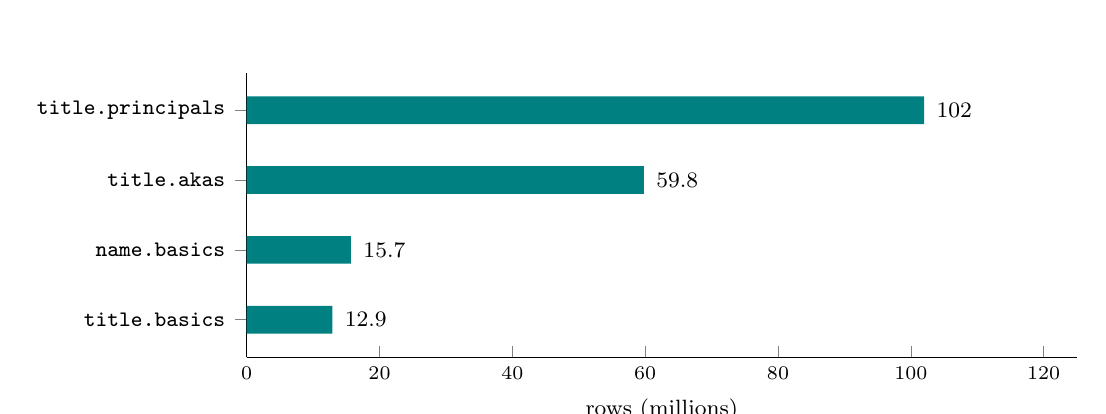
\begin{tikzpicture}
\begin{axis}[
  xbar, width=\textwidth, height=5.2cm,
  xmin=0, xmax=125,
  symbolic y coords={title.basics, name.basics, title.akas, title.principals},
  ytick=data, yticklabel style={font=\footnotesize\ttfamily},
  xlabel={rows (millions)}, xlabel style={font=\footnotesize},
  xticklabel style={font=\scriptsize},
  point meta=x, nodes near coords, nodes near coords style={font=\footnotesize\bfseries},
  every node near coord/.append style={xshift=1pt},
  bar width=10pt, enlarge y limits=0.18,
  axis x line*=bottom, axis y line*=left]
\addplot[fill=teal, draw=none] coordinates
  {(12.9,title.basics) (15.7,name.basics) (59.8,title.akas) (102,title.principals)};
\end{axis}
\end{tikzpicture}
\end{minipage}\hfill
\begin{minipage}[c]{0.4\textwidth}
\centering
\begin{tikzpicture}[node distance=5mm]
\node[dec] (age) {Pulled less than\\7 days ago?};
\node[src, draw=teal, below=of age, minimum width=34mm] (dl) {Download \code{.tsv.gz}\\\scriptsize\code{imdb/<file>/dt=<day>/}};
\node[src, draw=teal, below=of dl, minimum width=34mm] (cnt) {Stream-count rows\\\scriptsize 8\,MB chunks $\rightarrow$ manifest};
\node[dbx, below=of cnt, minimum width=34mm] (pr) {Prune old snapshot\\\scriptsize keep 1 (ratings: 2)};
\node[right=6mm of age, font=\footnotesize\itshape] (skip) {skip};
\draw[arr] (age) -- node[above, font=\scriptsize]{yes} (skip);
\draw[arr] (age) -- node[right, font=\scriptsize]{no} (dl);
\draw[arr] (dl) -- (cnt);
\draw[arr] (cnt) -- (pr);
\end{tikzpicture}
\end{minipage}
\caption{IMDb: rows per downloaded file (about 190 million in total), and the weekly pull flow.}
\label{fig:imdb}
\end{figure}

\begin{table}[H]
\centering\small
\begin{tabularx}{\textwidth}{@{}llXr@{}}
\toprule
Bronze table & IMDb file & Used for & Rows \\
\midrule
\code{imdb\_ratings} & \code{title.ratings} & Score and vote count & -- \\
\code{imdb\_titles} & \code{title.basics} & Title type, runtime & 12.9 M \\
\code{imdb\_principals} & \code{title.principals} & Directors, cast & 102 M \\
\code{imdb\_names} & \code{name.basics} & Names, professions & 15.7 M \\
\code{imdb\_akas} & \code{title.akas} & Localized titles (e.g.\ Vietnamese) & 59.8 M \\
\bottomrule
\end{tabularx}
\caption{IMDb files downloaded (about 1.5\,GB compressed).}
\end{table}

\begin{itemize}
  \item IMDb publishes \emph{full snapshots} with no incremental API. Each source is therefore downloaded at most once
        every 7 days (\code{IMDB\_MIN\_DAYS\_BETWEEN\_PULLS}) into \code{imdb/<file>/dt=<day>/}.
  \item Rows are counted by streaming the decompressed data in 8\,MB chunks, without extracting to disk (the
        uncompressed files are several GB).
  \item \textbf{Bounded snapshots}: \code{title.ratings} keeps 2 snapshots, the four large files keep 1. The function
        \code{prune\_imdb\_snapshots} removes the old snapshot's bronze rows, landing folder and manifest together, so
        reconciliation between bronze and manifests still matches.
  \item \code{title.crew} (duplicates \code{principals}) and \code{title.episode} (TV episodes) are not downloaded.
\end{itemize}

\subsection{TMDB API}
Notebook \code{05\_tmdb\_pull.py}, code \code{src/movie\_lakehouse/ingest/tmdb.py}.

\paragraph{Which movies.} Every \code{tmdb\_id} linked to a MovieLens movie (through \code{links.csv}) that at least one
sampled user has rated. Each movie is fetched with \code{/movie/\{id\}?append\_to\_response=videos,keywords} (details,
trailers and keywords in one request).

\paragraph{Fault-tolerant client.}
\begin{itemize}
  \item 16 threads (\code{ThreadPoolExecutor}) share one \code{RateLimiter} (at most 35 requests/second, below TMDB's
        limit).
  \item On network errors, HTTP 429 or 5xx: up to 6 retries, honouring the \code{Retry-After} header, otherwise a
        $2^{n}$-second backoff. When retries run out, status \code{599} is recorded so the next run tries again.
  \item The token lives in the Databricks secret scope \code{cinelake/tmdb\_token}, never in code or \code{.env}.
        The client accepts both the Read Access Token (Bearer) and the v3 API key.
\end{itemize}

\paragraph{Incremental.} Figure~\ref{fig:flow-tmdb} shows how each ID is handled.
\begin{enumerate}
  \item IDs that already have a final result (\code{200} or \code{404}) are skipped. Other statuses are retried.
  \item From the second run on, \code{state/tmdb\_pull.json} gives the date of the previous pull, and
        \code{/movie/changes} is queried (at most 14 days per query, paginated). Any changed ID that belongs to the
        catalog is fetched again.
  \item A JSONL file is written every 2,000 responses, so an interrupted job keeps what it already fetched.
\end{enumerate}

\begin{figure}[H]
\centering
\begin{tikzpicture}[node distance=7mm and 10mm]
\node[src, draw=teal] (ids) {\code{tmdb\_id} of every rated MovieLens movie};
\node[dec, below=of ids] (final) {Already 200\\or 404?};
\node[dec, below=of final] (chg) {In \code{/movie/changes}\\since last pull?};
\node[src, below=of chg] (skip) {Skip};
\node[box, fill=dark, text=white, right=18mm of chg, minimum width=44mm, minimum height=30mm] (get)
  {\textbf{GET /movie/\{id\}}\\+ videos, keywords\\16 threads $\cdot$ 35 req/s\\429/5xx $\rightarrow$ retry $\leq$ 6$\times$\\(Retry-After)};
\node[dbx, below=of get] (out) {\code{raw/tmdb/} JSONL every 2,000\\+ \code{state/tmdb\_pull.json}};
\draw[arr] (ids) -- (final);
\draw[arr] (final) -- node[right, font=\scriptsize]{yes} (chg);
\draw[arr] (chg) -- node[right, font=\scriptsize]{no} (skip);
\draw[arr] (final.east) -- node[above, font=\scriptsize, pos=0.3]{no} (final.east -| get.west);
\draw[arr] (chg) -- node[above, font=\scriptsize]{yes} (get);
\draw[arr] (get) -- (out);
\end{tikzpicture}
\caption{Flowchart: which TMDB movies are fetched on each run.}
\label{fig:flow-tmdb}
\end{figure}

\begin{lstlisting}[language=json, caption={One TMDB record on the landing zone (raw-first)}]
{"tmdb_id": "603", "fetched_at": "2026-10-18T02:11:05+00:00",
 "http_status": "200", "raw_json": "{\"id\": 603, \"title\": \"The Matrix\", ...}"}
\end{lstlisting}

\paragraph{Effect.} The first pull needed about 45 thousand requests and took 23 minutes. Later runs need only 211
requests (new IDs and IDs listed by \code{/changes}) and take 17 seconds (Figure~\ref{fig:tmdb-chart}).

\begin{figure}[H]
\centering
\begin{tikzpicture}
\begin{groupplot}[
  group style={group size=2 by 1, horizontal sep=2.2cm},
  ybar, width=6.5cm, height=5.5cm, ymode=log, log origin=infty,
  symbolic x coords={First pull, Incremental}, xtick=data,
  enlarge x limits=0.5, bar width=22pt,
  nodes near coords, nodes near coords style={font=\footnotesize\bfseries},
  point meta=rawy,
  every node near coord/.append style={/pgf/number format/fixed, /pgf/number format/1000 sep={,}},
  ticklabel style={font=\scriptsize}, title style={font=\small\bfseries},
  axis x line*=bottom, axis y line*=left]
\nextgroupplot[title={Requests (log scale)}, ymin=10, ymax=300000]
\addplot[fill=teal, draw=none] coordinates {(First pull,45000) (Incremental,211)};
\nextgroupplot[title={Wall time, seconds (log scale)}, ymin=1, ymax=10000]
\addplot[fill=amber, draw=none] coordinates {(First pull,1380) (Incremental,17)};
\end{groupplot}
\end{tikzpicture}
\caption{TMDB first pull vs.\ incremental run: about 200 times fewer requests, 80 times faster.}
\label{fig:tmdb-chart}
\end{figure}

\subsection{MovieLens 32M}
The zip file is downloaded once and extracted into 4 entities (\code{movies}, \code{ratings}, \code{tags},
\code{links}), each with a row-count manifest (header excluded). Since the manifest exists, later runs skip it.

% =====================================================================
\section{Demo}
% =====================================================================

The demo follows the three numbered paths of Figure~\ref{fig:kafka-arch}: \textcircled{\scriptsize 1} a rating in
the web app reaches Kafka within seconds, \textcircled{\scriptsize 2} the sink pushes it to Databricks as a JSONL
file, and \textcircled{\scriptsize 3} the external sources are pulled by Databricks.

\begin{figure}[H]
\centering
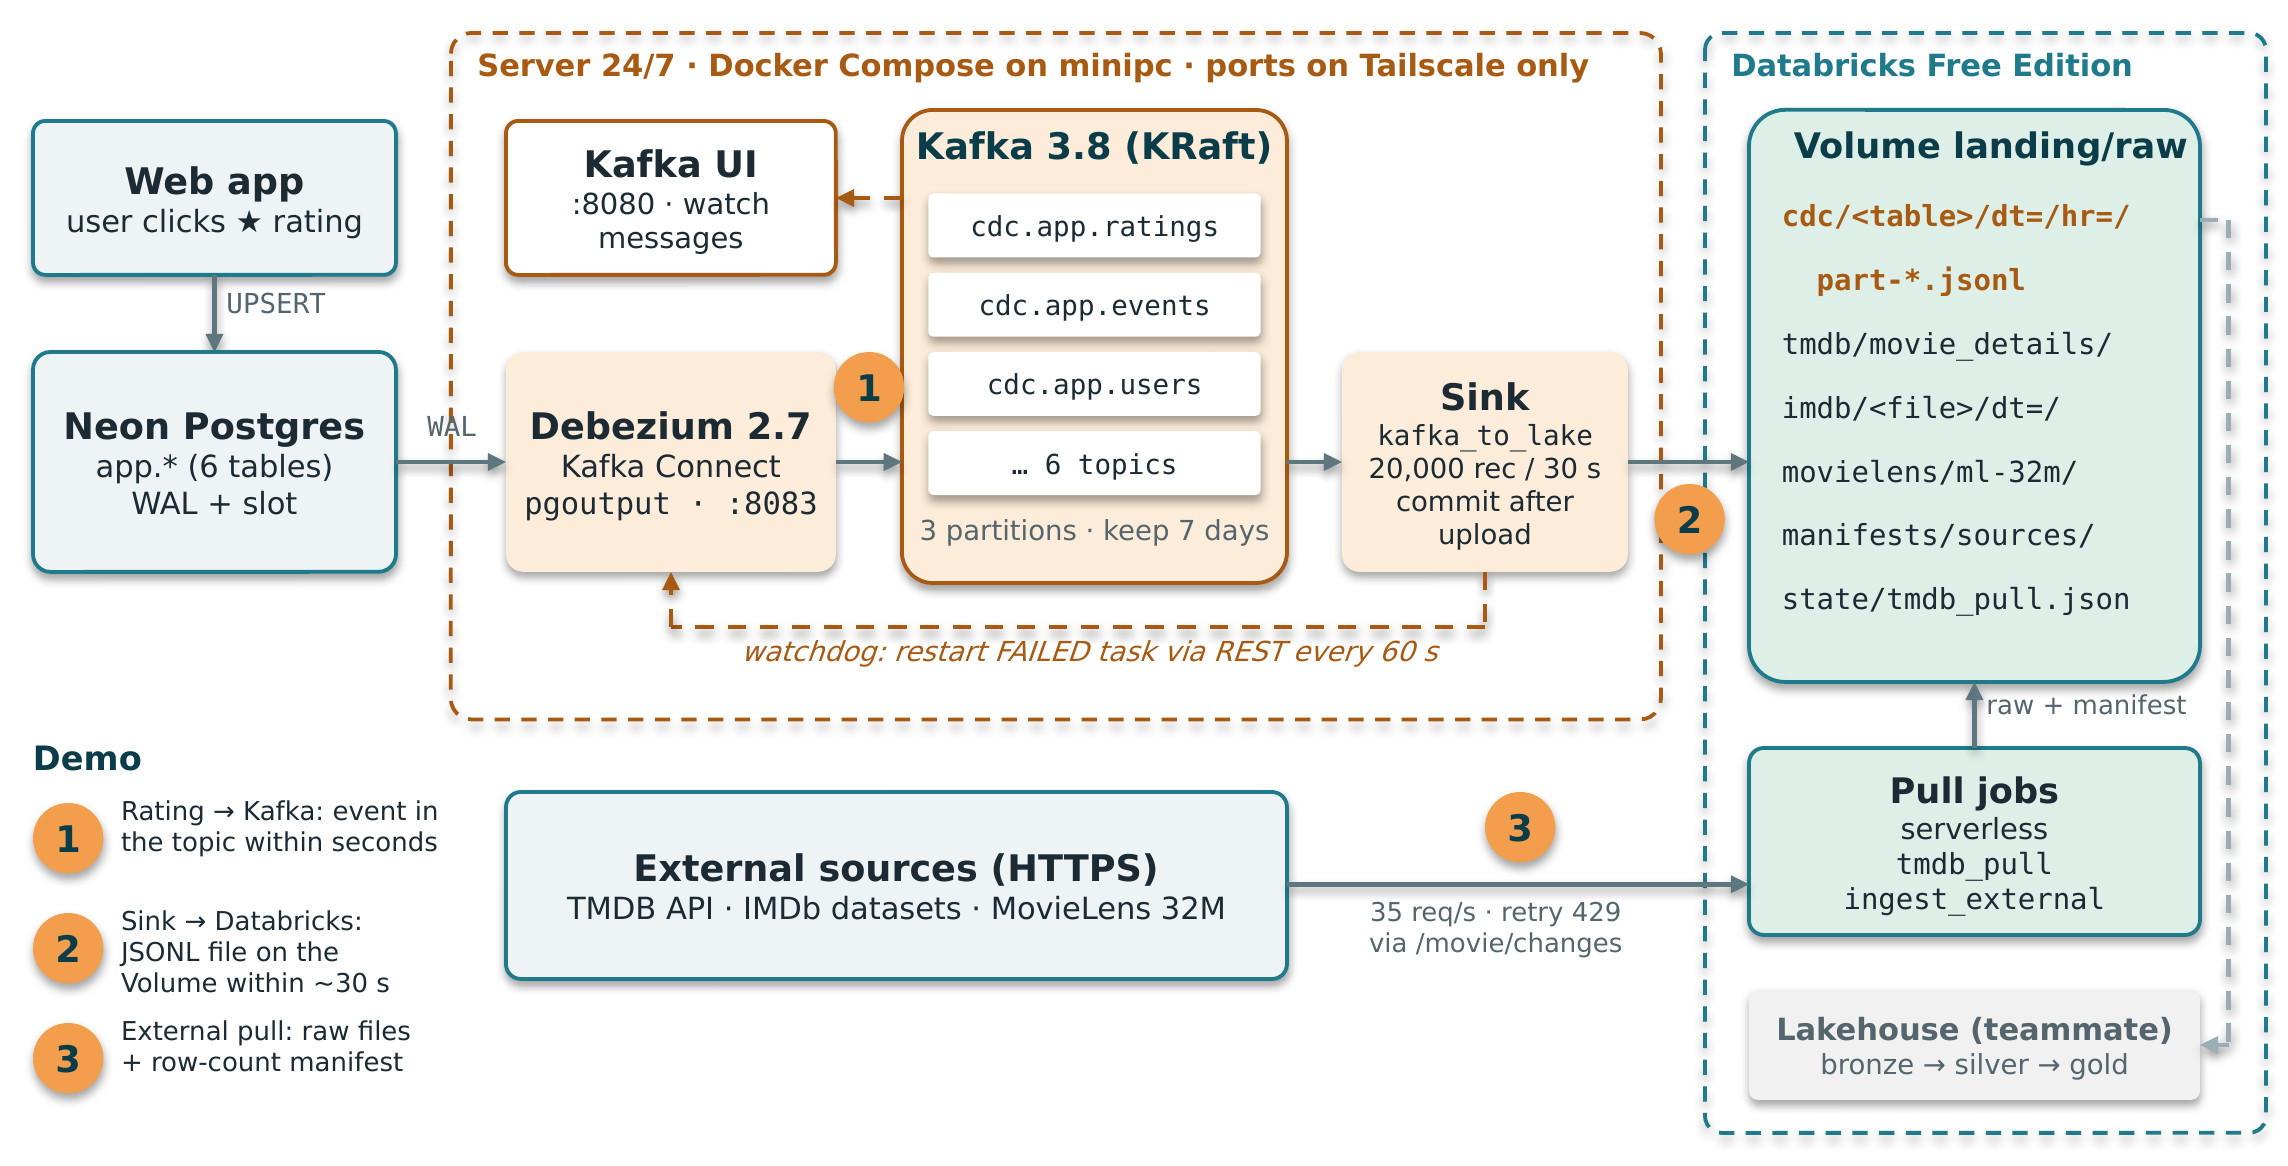
\includegraphics[width=0.9\textwidth]{figures/kafka-architecture.png}
\caption{Ingestion architecture around Kafka, with the three demo paths numbered.}
\label{fig:kafka-arch}
\end{figure}

\paragraph{Before the demo.} On the server, every service must be up and the connector running:
\begin{lstlisting}[language=bash, caption={Pre-demo checks on the server}]
docker compose ps                                  # kafka, connect, kafka-ui, sink: Up
.venv/bin/python -m ingestion.cdc.setup_cdc --status   # connector + task 0: RUNNING
docker compose logs -f sink                        # keep this open for demo 2
\end{lstlisting}

\subsection{Demo 1: a rating reaches Kafka within seconds}
\textbf{Goal}: show that a change in the app database is captured from the WAL and appears in Kafka almost
immediately, with no polling.
\begin{enumerate}
  \item Open Kafka UI (\code{http://<tailscale-ip>:8080}) $\rightarrow$ \emph{Topics} $\rightarrow$
        \code{cdc.app.ratings} $\rightarrow$ \emph{Messages}, sorted newest first.
  \item In the web app, rate a movie (or change an existing rating).
  \item Refresh Kafka UI: a new message appears. Point out \code{\_\_op} (\code{c} for a first rating, \code{u} for a
        re-rating), \code{\_\_lsn} and \code{\_\_source\_ts\_ms}.
  \item Compare \code{\_\_source\_ts\_ms} (commit time in Postgres) with the Kafka message timestamp shown by Kafka UI:
        the gap is in the order of milliseconds to a few seconds.
\end{enumerate}
\begin{lstlisting}[language=json, caption={A rating message as seen in Kafka UI and later in the JSONL file}]
{"user_id":185042,"movie_id":12429,"rating":"3.0","rated_at":"2026-11-07T16:48:49Z","source":"app",
 "created_at":"2026-11-07T18:03:00Z","updated_at":"2026-11-07T18:03:00Z",
 "__deleted":"false","__op":"c","__lsn":2274258168,"__source_ts_ms":1794074581487}
\end{lstlisting}
\textbf{What it proves}: log-based CDC catches every change as it is committed. Even when the app is idle, the
10-second heartbeat keeps the slot moving, so the next real change is not delayed by retained WAL.

\screenshot{figures/demo1-kafka-ui.png}{Demo 1: the new rating message in topic \code{cdc.app.ratings} (Kafka UI).}{fig:demo1}

\subsection{Demo 2: the sink pushes JSONL to Databricks}
\textbf{Goal}: show the micro-batch landing on the Volume, and that offsets are committed only after the upload.
\begin{enumerate}
  \item Watch the sink log. Within at most \code{flush-seconds} (30\,s) after the rating, a line appears:
\begin{lstlisting}[language=bash, numbers=none]
[sink] 1 records -> cdc/ratings/dt=2026-11-08/hr=15/part-20261108T152301-3f9c2a1b.jsonl (total ... in ... files)
\end{lstlisting}
  \item In Databricks, open \emph{Catalog} $\rightarrow$ \code{workspace.landing.raw} $\rightarrow$
        \code{cdc/ratings/dt=<today>/hr=<hour>/} and open the new file: one JSON line per change, identical to the
        Kafka message of demo 1.
  \item Optionally, query it directly from a notebook:
\begin{lstlisting}[language=SQL, numbers=none]
SELECT user_id, movie_id, rating, __op, __lsn, __source_ts_ms
FROM json.`/Volumes/workspace/landing/raw/cdc/ratings/dt=2026-11-08/`
ORDER BY __lsn DESC LIMIT 5;
\end{lstlisting}
  \item Optionally, \code{.venv/bin/python -m ingestion.trace --last 5} prints the timestamps of the change at every
        hop (commit, file on the Volume, and the lakehouse hops once the teammate's jobs have run).
\end{enumerate}
\textbf{What it proves}: the change lands as JSONL in under a minute; the file name contains a uuid, and offsets move
only after the file exists (Figure~\ref{fig:seq-cdc}, steps 8--10).

\screenshot{figures/demo2-volume-jsonl.png}{Demo 2: the sink log line and the JSONL file on the Volume.}{fig:demo2}

\subsection{Demo 3: pulling external sources}
\textbf{Goal}: show the pull path and its incremental behaviour.
\begin{enumerate}
  \item In the Databricks workspace, open notebook \code{05\_tmdb\_pull.py} and run it (widget \code{limit} can be set
        to a small number such as 200 for a short demo). The last cell prints the manifest of the run: number of
        requests, statuses and files written.
  \item Run it a second time: thanks to the skip rule and \code{/movie/changes}, it only fetches new or changed IDs
        (in production: 211 requests and 17 seconds instead of 45,000 and 23 minutes).
  \item Open notebook \code{02\_ingest\_external.py} and run it with \code{force=false}: IMDb and MovieLens are skipped
        because their manifests exist and the last IMDb pull is less than 7 days old.
  \item Show the result in \emph{Catalog}: \code{raw/tmdb/movie\_details/dt=<today>/part-*.jsonl},
        \code{state/tmdb\_pull.json}, and a manifest in \code{manifests/sources/} with its row counts.
\end{enumerate}
\textbf{What it proves}: external sources are stored raw, the pull is idempotent and incremental, and every pull leaves
a manifest that the lakehouse layer can reconcile against.

\screenshot{figures/demo3-tmdb-pull.png}{Demo 3: output of \code{tmdb\_pull} and the files and manifest it wrote.}{fig:demo3}

% =====================================================================
\section{Operations and handover}
% =====================================================================

\subsection{Handover to the lakehouse layer}
The ingestion layer ends at the landing zone. The lakehouse layer (bronze, silver, gold) is owned by a teammate and
reads files from \code{/Volumes/workspace/landing/raw/}. Both sides agree on a data contract (details in the handover
file \code{HANDOVER\_INGESTION\_TO\_LAKEHOUSE.md}):
\begin{itemize}
  \item \textbf{CDC}: each JSONL line is one change, with the table's columns (strings or numbers) plus
        \code{\_\_op} (\code{r}, \code{c}, \code{u}, \code{d}), \code{\_\_lsn}, \code{\_\_source\_ts\_ms}, \code{\_\_deleted}.
  \item \textbf{At-least-once delivery}: a change may appear more than once; the lakehouse dedups and orders by
        \code{\_\_lsn}.
  \item \textbf{Batch sources}: raw files plus a row-count manifest in \code{manifests/sources/} for reconciliation.
\end{itemize}

\subsection{Running 24/7}
The whole CDC part runs with Docker Compose (project \code{movie-lakehouse}) on \code{minipc}:
\begin{lstlisting}[language=bash, caption={Setup on the server}]
python3 -m venv .venv && .venv/bin/pip install -e ".[ingestion]"
docker compose up -d kafka connect kafka-ui
.venv/bin/python -m ingestion.cdc.setup_cdc --snapshot-mode no_data
docker compose --profile server up -d --build sink
\end{lstlisting}
\begin{itemize}
  \item Every service has \code{restart: unless-stopped}. Heap sizes are capped (Kafka 512\,MB, Connect 768\,MB) so the
        small machine keeps RAM for the sink and the daily jobs.
  \item New CDC files on the Volume fire the file-arrival trigger of job \code{cinelake\_refresh}
        (60 seconds after the last file, at least 6 hours between runs because of the Free Edition quota).
  \item A cron job at 01:00 runs \code{ingestion/simulator/run.py} (simulated behaviour through the app's own API, so
        it also flows through CDC), then \code{ingestion/retention.py}.
\end{itemize}

\subsection{Retention on Neon}
Neon Free has only 1\,GB, while \code{app.events} is an append-only log that keeps growing. \code{retention.py}
deletes events older than \code{RETENTION\_DAYS} (60 days) in batches of 50,000 rows so transactions stay short and
the WAL is streamed gradually, then runs \code{VACUUM}. The lakehouse still keeps the full history: in WAL order, an
event's INSERT always precedes its DELETE, and silver does not apply DELETEs of \code{app.events}.

\subsection{Checks and troubleshooting}
\begin{table}[H]
\centering\small
\begin{tabularx}{\textwidth}{@{}lXX@{}}
\toprule
Check & Command / where & Passes when \\
\midrule
Debezium & \code{python -m ingestion.cdc.setup\_cdc --status} & Connector and task \code{RUNNING} \\
Kafka & Kafka UI, topics \code{cdc.app.*} & New messages after each action in the app \\
Sink & \code{docker compose logs -f sink} & Line \code{[sink] N records -> cdc/<table>/...} \\
Volume & Catalog \code{workspace.landing.raw/cdc/} & New files every hour \\
End-to-end & \code{python -m ingestion.trace --last 5} & Every hop has a time, up to \code{serving.*} \\
\bottomrule
\end{tabularx}
\caption{Operations checklist.}
\end{table}

\begin{table}[H]
\centering\small
\begin{tabularx}{\textwidth}{@{}XX@{}}
\toprule
Symptom & Fix \\
\midrule
Debezium task \code{FAILED} & The watchdog restarts it every minute. If it keeps failing, check the \code{connect}
log and the network to Neon \\
Sink cannot log in to Databricks & Token expired: update \code{DATABRICKS\_TOKEN}, restart \code{sink} \\
Neon slot retains a lot of WAL & Connect has been down for long: start it. After several days, re-register with
\code{--snapshot-mode no\_data} \\
Two Debezium connectors on one slot & Only one connector may read \code{cinelake\_slot}: stop the old one before
registering a new one \\
\bottomrule
\end{tabularx}
\caption{Common incidents.}
\end{table}

% =====================================================================
\section{Evaluation}
% =====================================================================

\subsection{Data correctness}
\begin{itemize}
  \item \textbf{Manifest (R1)}: every batch file has an exact row count, so the lakehouse can reconcile after loading.
  \item \textbf{CDC reconciliation (R2)}: the number of rows replayed into Neon must equal the number of rows received
        through CDC (e.g.\ 597,897 = 597,897).
  \item \textbf{No loss, no duplicates}: offsets are committed only after the upload, combined with MERGE by LSN in
        silver.
\end{itemize}

\subsection{Latency}
\begin{table}[H]
\centering\small
\begin{tabularx}{\textwidth}{@{}lXl@{}}
\toprule
Segment & Nature & Latency \\
\midrule
Postgres $\rightarrow$ Debezium $\rightarrow$ Kafka & True streaming, change by change & Milliseconds to seconds \\
Kafka $\rightarrow$ Volume & Sink micro-batch (flush by size or time) & Under 1 minute \\
Volume $\rightarrow$ serving (lakehouse layer) & \code{availableNow} job on new files & About 12 minutes \\
\bottomrule
\end{tabularx}
\caption{Latency per segment (measured on the End-to-end trace page, 18/10/2026: 11.9 minutes from commit to serving).}
\end{table}

CDC latency is computed in silver as \code{\_ingested\_at} $-$ \code{\_source\_ts}. The \code{ingestion.trace} command
prints the time of one LSN at every hop and serves as evidence for the end-to-end demo.

\subsection{Pull efficiency}
\begin{itemize}
  \item TMDB incremental: from about 45,000 requests (23 minutes) on the first run down to 211 requests (17 seconds)
        on later runs (Figure~\ref{fig:tmdb-chart}).
  \item IMDb: at most once a week. Only 1 snapshot is kept for the four large files (about 190 million rows), so
        storage does not grow over time (Figure~\ref{fig:imdb}).
\end{itemize}

% =====================================================================
\section{Conclusion}
% =====================================================================

\paragraph{Results.} The ingestion layer brings all four kinds of sources (CSV, TSV, JSON API, CDC) into the lakehouse
under one principle: keep data raw, traceable and reconcilable. CDC runs 24/7 on the server: files are written before
offsets are committed (at-least-once, combined with the LSN for exactly-once), with a self-healing watchdog and least
privilege. API pulls tolerate network errors and rate limits, and are incremental and idempotent.

\paragraph{Limitations.}
\begin{itemize}
  \item One Kafka broker, replication factor 1: no tolerance to a hardware failure of the server (the Volume remains
        the long-term copy).
  \item Commit-to-serving latency of about 12 minutes, bounded by the Databricks Free Edition compute quota, not by CDC.
  \item IMDb has no incremental API, so each pull downloads a full snapshot again.
\end{itemize}

\paragraph{Future work.}
\begin{itemize}
  \item Multi-broker Kafka and a Schema Registry (Avro) to manage schema changes.
  \item A stream processor (Flink or continuous Structured Streaming) reading Kafka directly to refresh signals within
        seconds.
  \item More sources (OMDb, Trakt) following the same pattern: rate-limited client, raw storage, manifest.
\end{itemize}

\end{document}



\textit{To be completed: batch and incremental data flows
into Databricks.}

\subsection{Databricks Data Warehouse and Lakehouse Layer}

\textit{To be completed: how processing publishes data for
the user app and dashboard.
Section~\ref{sec:gold-dashboard-model} documents Gold inputs.}

\subsection{Administration Dashboard}
\label{sec:admin-dashboard}

The CineLake administration dashboard is specified as a Databricks
AI/BI dashboard backed by SQL datasets over \texttt{workspace.gold}.
It supports catalog management, discovery analysis, playback
monitoring, and user engagement reporting. The sections below define
the required outputs and how the dashboard will obtain and present
them.

\subsubsection{Dashboard Requirements}

\begingroup
\small
\setlength{\tabcolsep}{4pt}
\renewcommand{\arraystretch}{1.15}
\begin{longtable}{@{}>{\raggedright\arraybackslash}p{0.10\textwidth}
                    >{\raggedright\arraybackslash}p{0.28\textwidth}
                    >{\raggedright\arraybackslash}p{0.56\textwidth}@{}}
\caption{Requirements for the CineLake administration dashboard.}
\label{tab:admin-business-requirements}\\
\toprule
\textbf{ID} & \textbf{Requirement} & \textbf{Description}\\
\midrule
\endfirsthead
\toprule
\textbf{ID} & \textbf{Requirement} & \textbf{Description}\\
\midrule
\endhead
\bottomrule
\endfoot
AD-01 & Platform activity overview &
Display the latest 30-day activity indicators, the reporting timestamp,
and separate user and catalog totals.\\
AD-02 & Trending titles and movie performance &
Show published title rankings by time window and provide a title-level
view of play volume, completion, and ratings.\\
AD-03 & Discovery channel performance &
Compare detail-view volume and attributed plays, completions, and
ratings across discovery channels and reporting dates.\\
AD-04 & Search gap identification &
Rank normalized search terms by zero-result volume and surface
high-volume terms with low click-through.\\
AD-05 & Playback quality monitoring &
Compare startup latency, buffering, errors, and complaint volume by
device category and player version. Show playback volume alongside
quality measures.\\
AD-06 & Engagement and retention reporting &
Display user counts by engagement segment and monthly activity and
retention. Mark unpublished retention results as pending.\\
AD-07 & Watchlist outcome tracking &
Show saved titles, subsequent watches, completions and ratings, and
typical elapsed time between a save and a recorded outcome.\\
\end{longtable}
\endgroup

\subsubsection{Overview and Trending Titles}

\paragraph{AD-01. Platform activity overview.}
Select the most recent row of \texttt{mart\dbsep platform\dbsep kpis}
by ordering on \texttt{as\_of} and taking one row. Bind the active
user, active viewer, play, watch hour, completion, search, rating,
and feedback measures to KPI cards. Display \texttt{as\_of} alongside
the cards as the reference time for the rolling 30-day window. Place
total users, simulated users, and catalog titles in a separate group
because they describe the snapshot population. Label the 30-day
indicators as activity in the project dataset. The KPI mart combines
activity across account origins, so account filters apply only to
datasets with account-level breakdowns. The overview lets admins
assess platform activity before investigating a particular title,
discovery channel, or playback issue.

\begingroup
\small
\begin{verbatim}
SELECT as_of, active_users_30d, active_viewers_30d, plays_30d,
       watch_hours_30d, completion_rate_30d, searches_30d,
       ratings_30d, avg_rating_30d, feedback_30d, new_users_30d,
       total_users, simulated_users, catalog_titles
FROM workspace.gold.mart_platform_kpis
ORDER BY as_of DESC
LIMIT 1;
\end{verbatim}
\endgroup

\paragraph{AD-02. Trending titles and movie performance.}
Filter \texttt{mart\dbsep trending\dbsep movies} by the selected
\texttt{window\_days} value of 1, 7, or 30. Sort by the published rank
and display title, plays, ratings, unique raters, and average rating
in a ranked table. Use \texttt{movie\_id} to retrieve the selected
title from \texttt{mart\dbsep movie\dbsep catalog}, including catalog
status, completion rate, play volume, and viewing hours. The ranking
filter applies to the ranking dataset. Label catalog metrics with
their own coverage and use a fact-level query when both measures
must share a specific date window. Admins can prioritize popular
titles that also have low completion and inspect them on the
playback quality page.

\subsubsection{Discovery and Search}

\paragraph{AD-03. Discovery channel performance.}
Read \texttt{mart\dbsep discovery\dbsep funnel} at its date and
discovery-source reporting grain. Apply the date and channel filters
to this dataset and plot daily detail views by source. Use a grouped
chart or table for detail views with attributed plays, completions,
and ratings. Keep the outcome series separate pending confirmation
of how the transformation attributes outcomes and whether they form
a sequence. Sum counts when aggregating across disjoint groups.
Any rate for a broader selection requires its own eligible numerator
and denominator. The comparison helps admins locate channels that
generate substantial browsing activity but few recorded follow-up
actions.

\paragraph{AD-04. Search gap identification.}
Read \texttt{mart\dbsep search\dbsep gaps} at normalized-query grain.
Show the query, search volume, zero-result count, published
click-through rate, and latest search timestamp. Sort the default
table by zero-result volume and use a minimum search count for
low click-through comparisons. For a selected reporting period,
filter \texttt{fact\dbsep search} on \texttt{searched\_at} before
grouping by \texttt{normalized\_query}. Count searches with
\texttt{results\_count = 0}. For a zero-result rate, divide by the
number of searches with a known result count. When calculating a
recorded-click rate directly, count searches with a non-null
\texttt{clicked\_movie\_id} and divide by the number of searches in
the filtered group. The table gives catalog admins a prioritized
list of terms to check for missing titles, title aliases, or poor
result relevance.

\begingroup
\small
\begin{verbatim}
SELECT normalized_query, searches, zero_result_searches,
       click_through_rate, last_searched_at
FROM workspace.gold.mart_search_gaps
WHERE zero_result_searches > 0
ORDER BY zero_result_searches DESC, searches DESC,
         normalized_query
LIMIT 25;
\end{verbatim}
\endgroup

\subsubsection{Playback Quality}

\paragraph{AD-05. Playback quality monitoring.}
Select date, device category, player version, plays, startup p50
and p95, buffering, errors, and complaints from
\texttt{mart\dbsep playback\dbsep quality}. Keep the date, device,
and version grain for the daily startup and error trends. Pair each
trend with playback volume so a group with very few plays is visible.
For a selected movie, filter \texttt{fact\dbsep playback} on its
\texttt{movie\_id} and the playback start time. Group by device
category and player version. Compute startup p95 from the eligible
\texttt{startup\_ms} values and report the number of non-null samples.
To obtain a percentile across multiple days or groups, compute it
from the underlying startup measurements for the selected population.

For feedback categories, group \texttt{fact\dbsep feedback} by
\texttt{category} and count feedback events. To relate feedback to
playback, verify the join on \texttt{playback\_id} and aggregate
feedback to playback grain before combining the measures. These views
help engineers identify devices or versions with elevated startup
latency or errors and prioritize the combinations with the greatest
playback volume.

\subsubsection{Engagement and Watchlists}

\paragraph{AD-06. Engagement and retention reporting.}
Group \texttt{mart\dbsep user\dbsep engagement} by \texttt{segment}
and, where selected, \texttt{user\_source}. Count users and show
the results in a segment bar chart. Use \texttt{is\_simulated} to
provide simulator context for this dataset. Plot
\texttt{mart\dbsep user\dbsep retention} by \texttt{month}, with
active and new user counts available alongside the retention trend.
For a finalized month, the published rate is consistent with
\texttt{retained\_users} divided by \texttt{active\_users} in that
same reported month. Show a pending state when \texttt{is\_final}
is false. The engagement breakdown helps admins understand the
composition of the active and dormant populations. The retention
series shows whether return activity changes over successive
finalized months.

\begingroup
\small
\begin{verbatim}
SELECT month, active_users, new_users, retained_users,
       CASE WHEN is_final THEN retention_rate END AS final_rate,
       is_final
FROM workspace.gold.mart_user_retention
ORDER BY month;
\end{verbatim}
\endgroup

\paragraph{AD-07. Watchlist outcome tracking.}
Read \texttt{mart\dbsep watchlist\dbsep conversion} at movie grain.
Show title, saves, savers, watched after save, completed after save,
rated after save, and average days to each timed outcome in a ranked
table. Use movie and minimum-save filters for comparisons. Display
each outcome independently because several outcomes may apply to the
same saved pair. A date filter for save cohorts requires
\texttt{fact\dbsep watchlist.added\_at}. Apply the same follow-up
window to each cohort before comparing outcome rates. A combined
conversion rate requires the Gold transformation's documented
eligibility and outcome rules. Admins can use this view to identify
movies with frequent saves but limited follow-through and inspect
whether that pattern is concentrated in recently saved entries.

\subsubsection{Refresh and Validation}

Refresh the SQL datasets after Gold has been published. Display the
reporting reference and, where available, the dashboard refresh time
as separate timestamps. Each filter applies to datasets that contain
its reporting field. Display undefined rates as unavailable.

Validate the cards and tables against SQL run over the same Gold
publication. Reference outputs from the profiled dataset include
3,848 active users, 2,427 active viewers, 7,489 plays, 11,210.05
watch hours, and 66.6\% completion in the KPI window. In the
retention dataset, 2,048 retained users out of 3,180 active users
reproduce the published September rate of 64.4\%. The subsequent
October and November rows are pending in that dataset. These values
are reconciliation examples for the recorded dataset.

For the end-to-end demonstration, record a known movie detail-view
or playback event. Locate its identifier in the corresponding Gold
fact, check the applicable mart after publication, and reconcile
the displayed measure after refreshing the dashboard. Confirm the
qualifying retention activity and return window, discovery
attribution, and combined watchlist conversion rules with the
Gold transformation before assigning those measures more specific
business labels.

\end{document}